\documentclass[11pt,a4paper]{article}
% Generated by research/unified/build.py from the empirical and theory sources.
\usepackage[margin=25mm]{geometry}
\usepackage[utf8]{inputenc}
\usepackage{amsmath,amssymb,amsthm,mathtools,graphicx,booktabs,longtable,tabularx,array}
\usepackage{xcolor,microtype,hyperref,fancyvrb,enumitem}
\usepackage[numbers,sort&compress]{natbib}
\hypersetup{colorlinks=true,linkcolor=blue!50!black,urlcolor=blue!50!black}
\setlength{\emergencystretch}{3em}
\setlength{\parskip}{4pt}
\newtheorem{theorem}{Theorem}[section]
\newtheorem{lemma}[theorem]{Lemma}
\newtheorem{proposition}[theorem]{Proposition}
\newtheorem{corollary}[theorem]{Corollary}
\theoremstyle{definition}
\newtheorem{definition}[theorem]{Definition}
\newtheorem{assumption}[theorem]{Assumption}
\theoremstyle{remark}
\newtheorem{remark}[theorem]{Remark}
\newcommand{\E}{\mathbb E}
\newcommand{\R}{\mathbb R}
\newcommand{\norm}[1]{\left\lVert#1\right\rVert}
\newcommand{\ip}[2]{\left\langle#1,#2\right\rangle}
\newcommand{\diag}{\operatorname{diag}}
\newcommand{\sigmoid}{\operatorname{sigmoid}}
\newcommand{\clip}{\operatorname{clip}}
\newcommand{\sgn}{\operatorname{sign}}
\title{PsiLogic: Chaos-Aware Active Cancellation for Adam\\\large Implementation, Convergence Theory, and Cross-Domain Benchmarks}
\author{\textbf{Ali Sultonov}\\Independent Researcher\\troxtergrif@gmail.com\\\url{https://github.com/Troxter222/psilogic}}
\date{}

\hypersetup{pdftitle={PsiLogic: Implementation, Convergence Theory, and Cross-Domain Benchmarks},pdfauthor={Ali Sultonov},pdfsubject={Unified empirical article and complete conditional convergence proofs}}

\begin{document}
\maketitle
\textbf{Original publication:} arXiv:2607.16268v1 [cs.LG], first submitted 5 July 2026. \url{https://arxiv.org/pdf/2607.16268}.

\textbf{Article DOI:} \url{https://doi.org/10.48550/arXiv.2607.16268}.

Unified local revision: implementation and empirical audit of 15 October 2026, with convergence theory and complete proofs integrated on 16 October 2026. Audited software version: 0.6.0.

\begin{abstract}

PsiLogic multiplies an Adam-style update by a bounded, tensor-specific trust factor. The factor combines changes in a normalized gradient norm with disagreement between the current gradient and previous momentum. We state the equations implemented in the current source, including preprocessing, bias correction, epsilon placement, warmup, and optional update modes. Here, ``chaos'' names a gradient statistic; it is not a claim about mathematical chaos or a direct measurement of training instability.

We reassess two saved H100 benchmark snapshots. The four-task reference snapshot favors PsiLogic in mean NLP perplexity and ViT accuracy. The later partial snapshot gives a different picture: NLP perplexity is 8.15 \(\pm\) 0.16 for PsiLogic and 8.20 \(\pm\) 0.20 for AdamW; ViT accuracy is 26.72 \(\pm\) 0.67\% and 28.25 \(\pm\) 0.47\%; ResNet accuracy is 22.08 \(\pm\) 0.23\% and 22.14 \(\pm\) 0.52\%. Recorded run wall time in the later snapshot is 1.099\(\times\), 1.024\(\times\), and 1.038\(\times\) AdamW, respectively. No later diffusion outcome is available. These are run-time ratios; a separate saved optimizer-only microbenchmark reports a fused-step ratio of 2.27\(\times\) AdamW. The snapshots use different software versions and selected learning rates, so their difference does not isolate kernel fusion. We report seed-paired tests with an explicit Holm correction and retain the older results separately. No new training was performed for this revision. The evidence supports modest full-run overhead in the later workloads, but does not establish a general quality advantage over AdamW or validate every historical outcome for the current implementation.


The convergence analysis retains the full implemented detector, both Adam
moments, bias correction, and the actual epsilon convention. Under explicit
bounded-gradient and small-step assumptions, with parameter decay and gradient
preprocessing disabled, it proves a pathwise stationarity-energy bound and
$O(T^{-1})$ average squared gradient for deterministic gradients. Stochastic
conclusions require controlled oracle error. Counterexamples identify failures
of broader claims, and ten scalar and finite-sum lemmas are kernel-checked in
Lean 4. These guarantees do not certify the benchmark configurations or
establish an unconditional advantage over AdamW.

\end{abstract}

\section{Motivation and scope}

Adam already adapts its update through running gradient moments \citep{kingma2015adam}. PsiLogic asks a narrower question: can a small additional reduction of each tensor's update help when recent gradient statistics change or its gradient opposes accumulated momentum? It keeps Adam's coordinate-wise preconditioner and adds one scalar multiplier per tensor. Tensors can receive different damping even when they share a learning rate.

This motivation does not establish better training. A gradient opposing momentum may contain useful information, and damping it may slow progress. A sudden norm increase may also be meaningful rather than harmful. We treat the detector as a heuristic rather than calling it a reliable measure of confusion or convergence.

This manuscript revises the original PsiLogic preprint \citep{psilogic2026preprint}, first submitted to arXiv on 5 July 2026. The arXiv paper is the primary scholarly reference for PsiLogic. This local revision makes the current update explicit and reports what the saved measurements support, including unfavorable outcomes. These are distinct evidence: run metadata does not identify exact training commits or serialize every resolved optimizer setting. Equations describe the audited source; tables describe named CSV snapshots. We cannot certify that an archived run executed every equation of today's implementation.

\section{Relation to existing optimizers}

Adam maintains first and second moments and corrects their initialization bias \citep{kingma2015adam}. AdamW separates parameter decay from the gradient direction \citep{loshchilov2019decoupled}. PsiLogic follows that separation: ordinary decay acts on parameters, while cancellation scales the optimizer update. Optional Lion mode uses a sign-momentum direction \citep{chen2023lion} with the same trust factor. This is a tensor-level effective learning-rate adjustment, not a curvature estimate or replacement for an external schedule.

Gradient centralization and adaptive gradient clipping are optional preprocessing operations. They change the gradients used by both optimizer and detector. Results with these options enabled measure the full configuration and cannot isolate cancellation's contribution. We make no claim of priority over all gradient-dependent learning-rate methods. Section~\ref{sec:convergence} establishes conditional convergence guarantees for a precisely specified Adam configuration and states the modes and noise regimes they exclude.

\section{The implemented algorithm}\label{sec:implemented}

\subsection{State and preprocessing}

Let $i$ identify a tensor in parameter group $k$, and $n_i$ its number of elements. Its counter $t$ starts at 1 and advances only when that tensor has a gradient. A skipped tensor receives no moment, detector, or decay update. Thus $t$ need not equal the global step. Let $\eta_{k,t}$ be the trainer-supplied learning rate, $\lambda_k$ the decoupled decay coefficient, and $\epsilon$ the numerical stabilizer. We suppress group indices on other settings. Parameter-shaped products, squares, square roots, and divisions are elementwise.

Let $h_{i,t}$ be the gradient received by the optimizer, after trainer-side unscaling, accumulation, or global clipping. Tensor-wise adaptive gradient clipping (AGC) with coefficient $a>0$ gives

\[
\widetilde g_{i,t}=h_{i,t}\min\left(1,\frac{a\max(\|\theta_{i,t}\|_2,10^{-3})}{\max(\|h_{i,t}\|_2,10^{-6})}\right).
\]

For $a\leq0$, $\widetilde g=h$. Enabled gradient centralization, on tensors with more than one dimension, gives

\[
g_{i,t}=\widetilde g_{i,t}-\operatorname{mean}_{d=1,\ldots,D_i-1}(\widetilde g_{i,t}).
\]

Otherwise $g=\widetilde g$. Reduced dimensions remain for broadcasting; the first dimension is not averaged. Moments and detector use $g$. Secondary decay uses $\widetilde g$ before centralization. AGC reads parameters before decay. State is FP32 even with \path{FP16/BF16} parameters. Equations specify arithmetic, not bitwise equality across devices or dtypes.

\subsection{Normalized gradient statistics}

The root-mean-square gradient magnitude is

\[
u_{i,t}=\frac{\|g_{i,t}\|_2}{\sqrt{\max(n_i,1)}}.
\]

Initialize $A_{i,1}=u_{i,1}$ and dimensionless averages $F_{i,1}=S_{i,1}=1$. For $t>1$,

\[
\begin{aligned}
A_{i,t}&=0.99A_{i,t-1}+0.01u_{i,t},\\
r_{i,t}&=u_{i,t}/(A_{i,t}+\epsilon),\\
F_{i,t}&=0.90F_{i,t-1}+0.10r_{i,t},\\
S_{i,t}&=0.99S_{i,t-1}+0.01r_{i,t}.
\end{aligned}
\]

The ratio uses newly updated $A$. Averages advance during warmup and with cancellation disabled. They track relative magnitude, not gradient variance. Normalization approximately removes constant gradient rescaling when epsilon is negligible; it is not exact scale invariance near numerical zero.

\subsection{Continuous signal and trust}

With momentum before the current update denoted by $m_{i,t-1}$, set disagreement $D_{i,1}=0$. Subsequently,

\[
\begin{aligned}
c_{i,t}&=\operatorname{clip}\left(\frac{\langle m_{i,t-1},g_{i,t}\rangle}{\|m_{i,t-1}\|_2\|g_{i,t}\|_2+\epsilon},-1,1\right),\\
D_{i,t}&=\tfrac12(1-c_{i,t}).
\end{aligned}
\]

Epsilon is inside the cosine denominator. After the first update, zero momentum or zero gradient gives $D=1/2$, not the first-step value. With $\sigma(x)=1/(1+e^{-x})$, adaptive scale $\tau_s$ and fixed setting $\tau_c$, define

\[
E_{i,t}=\begin{cases}
\sigma\left(\dfrac{4}{\max(\tau_s-1,0.25)}\left(\dfrac{F_{i,t}}{S_{i,t}+\epsilon}-1\right)\right),&\text{adaptive},\\
\sigma\left(4\left(\dfrac{S_{i,t}}{\max(\tau_c,\epsilon)}-1\right)\right),&\text{fixed}.
\end{cases}
\]

Fixed mode also uses normalized slow state, not a raw-norm threshold. When the cancellation path is active,

\[
C_{i,t}=\tanh(S_{i,t})\left(\tfrac12 E_{i,t}+\tfrac12 D_{i,t}\right).
\]

With warmup gain $w$, effective gamma $\gamma$, amplification $P_k$, and $b=\min(b_0,0.99)$,

\[
T_{i,t}=1-\min(C_{i,t}\gamma_{i,t}P_k w_{i,t},b).
\]

For intended nonnegative amplification, $1-b\leq T\leq1$. Default $b_0=0.05$ gives $T\geq0.95$. The code clamps cancellation only from above and does not reject negative amplification; these bounds assume $P_k\geq0$.

If gain or effective gamma is zero, the path is inactive: trust is 1 and the stored soft signal is zero. This is an inactive marker, not a measurement of quiet gradients. Equal fast and slow state does not close the gate: their ratio near 1 gives $E\approx1/2$. With $S\approx1$ and aligned gradients, $C\approx\tanh(1)/4\approx0.1904$. Gamma 0.05, amplification 1, and full gain then yield about 0.95\% damping. Stable directions and small absolute gradients do not guarantee zero cancellation; a limit such as $S\to0$ does force the active signal to zero.

\subsection{Schedules and warmup}

For configured horizon $H$, the common gamma and secondary-decay schedule is

\[
z_t=\begin{cases}\tfrac12[1+\cos(\pi\min(t/H,1))],&H>0,\\1,&H=0.\end{cases}
\]

Set $\gamma_t^{\rm sched}=\gamma_0z_t$ and $q_t=q_0z_t$. Optional automatic gamma multiplies scheduled gamma by $\max(S_{i,t}/0.1,0.1)$ when $t>1$ and $S_{i,t}<0.1$, and leaves it unchanged otherwise. This option is off by default and is not a convergence test.

Automatic chaos warmup gives $W=\max(500,\lfloor H/20\rfloor)$ for $H>0$, or 200 for $H=0$. An explicitly supplied nonnegative length overrides it. With $R=\max(1,\lfloor W/4\rfloor)$,

\[
w_{i,t}=\begin{cases}0,&t\leq W,\\\min(1,(t-W)/R),&t>W.\end{cases}
\]

Warmup zero activates the path on the first update. The bare constructor with unknown horizon waits 200 updates, then ramps for 50. This is separate from trainer LR warmup. Each tensor's counter drives both internal schedules.

\subsection{Adam update, epsilon, and decay}

Starting with $m_{i,0}=v_{i,0}=0$,

\[
\begin{aligned}
m_{i,t}&=\beta_1m_{i,t-1}+(1-\beta_1)g_{i,t},\\
v_{i,t}&=\beta_2v_{i,t-1}+(1-\beta_2)g_{i,t}^{\odot2}.
\end{aligned}
\]

Ordinary decay multiplies parameters by $1-\eta_{k,t}\lambda_k$. If $q_t>0$ and cancellation is active ($w>0$, $\gamma>0$), secondary decay adds

\[
\rho_{i,t}=1-\eta_{k,t}q_tw_{i,t}(1-C_{i,t})\tanh(|\widetilde g_{i,t}|).
\]

Otherwise $\rho=1$. The API calls this option quantum\_decay; it has no quantum-mechanical interpretation and is disabled by default. Both decay factors act before the optimizer direction:

\[
\boxed{\theta_{i,t+1}=\rho_{i,t}(1-\eta_{k,t}\lambda_k)\theta_{i,t}
-\eta_{k,t}\frac{\sqrt{1-\beta_2^t}}{1-\beta_1^t}\,T_{i,t}\frac{m_{i,t}}{\sqrt{v_{i,t}}+\epsilon}.}
\]

With bias-corrected moments $\widehat m=m/(1-\beta_1^t)$ and $\widehat v=v/(1-\beta_2^t)$, the direction is

\[
\frac{T_{i,t}\widehat m_{i,t}}{\sqrt{\widehat v_{i,t}}+\epsilon/\sqrt{1-\beta_2^t}}.
\]

Replacing that denominator with $\sqrt{\widehat v}+\epsilon$ changes the algorithm. For $\beta_2=0.999$, first-update effective epsilon is about $31.62\epsilon$. With all extras disabled, this is AdamW-style arithmetic with that convention, not exact algebraic identity to usual PyTorch AdamW. Tolerance-based equivalence checks do not prove exact equality.

\subsection{Lion and distributed execution}

Optional Lion mode gives

\[
\begin{aligned}
d_{i,t}&=\operatorname{sign}(\beta_1m_{i,t-1}+(1-\beta_1)g_{i,t}),\\
\theta_{i,t+1}&=\rho_{i,t}(1-\eta_{k,t}\lambda_k)\theta_{i,t}-\eta_{k,t}T_{i,t}d_{i,t},\\
m_{i,t}&=\beta_2m_{i,t-1}+(1-\beta_2)g_{i,t}.
\end{aligned}
\]

Disagreement still uses previous momentum. Lion has no Adam bias correction. The shared initializer allocates a second-moment buffer, but it does not enter this update.

Optional distributed detector synchronization averages $F,S$ across ranks after their local update and before computing the signal. It does not explicitly synchronize $A$ or disagreement. Averaging $F,S$ cannot guarantee identical trust if ranks differ in gradients, momentum, counters, or settings. Ordinary DDP with matching reduced gradients and state is the intended setting.

\subsection{Execution order, defaults, and source map}

\begin{enumerate}[itemsep=2pt]
\item Skip tensors without gradients; apply optional AGC, then centralization.
\item Increment active tensor counters; when cancellation can activate, compute disagreement against previous momentum.
\item Update Adam moments in Adam mode and norm averages in both modes.
\item Optionally average \path{fast/slow} state across distributed ranks.
\item Resolve effective gamma, signal, and trust. Apply ordinary decay, then active secondary decay.
\item Apply the direction; update Lion momentum after constructing its direction.
\end{enumerate}

Bare defaults are LR 0.001, betas (0.9, 0.999), decay 0.0001, epsilon 1e-8, gamma 0.05, amplification 1, cap 0.05, adaptive thresholding, tau scale 2, and automatic chaos warmup. AGC, centralization, secondary decay, automatic gamma, Lion, and detector synchronization are off. CUDA foreach and fused execution are requested by default with availability-dependent fallback. CPU and compilation use the scalar implementation. Presets and parameter groups can override these settings.

API mapping: $A,F,S$ are gn\_avg, fast, slow; $C$ is soft\_chaos; $P_k$ is p\_ext; $b_0$ is max\_cancel; $\tau_s,\tau_c$ are tau\_scale, chaos\_tau; $H$ is gamma\_T\_max; $q_0$ is quantum\_decay; $a$ is agc\_clip. Preprocessing and update order are in \path{psilogic/optimizer.py}; detector helpers in \path{psilogic/_chaos.py}; accelerated execution in \path{psilogic/_cuda/step.py} and kernels.py. Backends target the same rule, with possible precision and reduction-order differences. Software checks cannot establish which source a historical run executed.


\section{Convergence Theory and Proofs}\label{sec:convergence}
This section supplies the complete conditional convergence analysis for the
update described in Section~\ref{sec:implemented}. It is placed before the
empirical protocol to make the mathematical guarantee and its limits explicit
before the benchmark results are interpreted. The deterministic guarantee,
stochastic error bounds, and counterexamples concern precisely stated
configurations; they do not validate every benchmark preset.

For the proofs, $x_t$ concatenates the parameter tensors $\theta_{i,t}$,
$u_t^{(b)}$ denotes the trust $T_{i,t}$, and $s_t$ denotes the soft signal
$C_{i,t}$ of the implementation section. The notation $h_t=\nabla f(x_t)$
means the true objective gradient here; the earlier implementation notation
$h_{i,t}$ meant the received raw gradient. This distinction is needed to state
oracle error. The recurrence below restates the same algorithm in this proof
notation, preserving its epsilon convention and update order. All sidecar
filenames and the \texttt{lean/} directory named in this section are relative
to \path{research/convergence/}.
\setlength{\parskip}{0pt}
\numberwithin{equation}{section}
\subsection{Scope and mathematical contributions}
Adaptive normalization and momentum are useful algorithmic mechanisms, but
neither positive step multipliers nor small empirical loss establish a
convergence theorem. PsiLogic adds a multiplier computed from the same gradient
used in its update. This creates a conditional dependence that must be retained
in the analysis. The present object of study is the local package at revision
\texttt{b4917163d63d8a5cb2960e29af4b1bccdbf5798d}, with its working-tree state
recorded in \texttt{source\_snapshot.json}. Existing papers, documentation, and
release equations were not used as the algorithm specification.

The main contributions are: (i) exact equations and branch coverage;
(ii) uniform real-arithmetic bounds on the implemented detector;
(iii) a pathwise error-energy theorem for bias-corrected momentum with arbitrary,
possibly current-gradient-dependent, uniformly positive diagonal scaling;
(iv) its specialization to an actual PsiLogic configuration, with explicit
constants; and (v) counterexamples defining the limits of stronger claims.
The main theorem does not assume monotonic second moments, independence of
trust and gradients, or the convergence of classical Adam. Its sufficient step
bound can be extremely conservative when epsilon is small. It is a rigorous
existence guarantee, not a recommendation for training hyperparameters.

\subsection{Notation and recurrence for the proofs}\label{sec:algorithm}
\subsubsection{Blocks, clocks, defaults, and preprocessing}
Partition $x\in\R^d$ into parameter tensors $x^{(b)}\in\R^{d_b}$; tensor shape
is retained for centralization. A block with \texttt{grad is None} receives no
update, no decay, and no local-clock increment. In this section $k\ge1$ is a
block's local active-update count; $x$ denotes its pre-step value. Group options
may differ. Unless otherwise specified, all formulas are exact-real
interpretations, not statements about floating-point evaluation.

The constructor defaults are
\[
\begin{gathered}
\eta=10^{-3},\quad (\beta_1,\beta_2)=(0.9,0.999),\quad
\lambda=10^{-4},\quad \gamma=0.05,\quad p_{\rm ext}=1,\\
q=0,\quad \epsilon=10^{-8},\quad c_{\max}=0.05,\quad
\tau=0.5,\quad \tau_{\rm scale}=2,\quad H=0,\quad W_{\rm cfg}=-1.
\end{gathered}
\]
AGC, centralization, Lion, auto-gamma, and DDP chaos synchronization default to
false (AGC coefficient zero); adaptive thresholding, foreach, and fused CUDA
selection default to true. Task presets and parameter-group builders can
change these choices. No global norm clipping is implemented by this optimizer;
external training-loop clipping is outside its update path.

Given raw supplied gradient $z$, AGC with coefficient $a_{\rm gc}>0$ computes
\begin{equation}\label{eq:agc}
\chi=\min\left\{1,
\frac{a_{\rm gc}\max(\norm{x},10^{-3})}{\max(\norm{z},10^{-6})}\right\},
\qquad r=\chi z.
\end{equation}
With AGC disabled, $r=z$. Centralization gives $g=Pr$, where $P$ subtracts the
mean over every axis except the leading axis if tensor rank exceeds one;
otherwise $P=I$. All moments and detector norms use $g$. Quantum decay uses
$r$, specifically \emph{after AGC and before centralization}. The norm in
\eqref{eq:agc} is a whole-tensor Euclidean norm, not a per-row norm.

\subsubsection{Detector, schedules, and cancellation}
The initialized state is $m_0=v_0=0$, $A_0=F_0=S_0=0$, stored soft chaos zero,
and local count zero. Moments are block vectors; $A,F,S$ and soft chaos are
one-element tensors. Define $R_k=\norm{g_k}/\sqrt{\max(d_b,1)}$. At the first
active step,
\begin{equation}\label{eq:seed}
 A_1=R_1,\qquad F_1=S_1=1,
\end{equation}
even when $g_1=0$. At later steps,
\begin{equation}\label{eq:ema}
 A_k=.99 A_{k-1}+.01R_k,\quad Z_k=\frac{R_k}{A_k+\epsilon},\quad
 F_k=.9F_{k-1}+.1Z_k,\quad S_k=.99S_{k-1}+.01Z_k.
\end{equation}
If enabled and a process group exists, DDP replaces $F_k,S_k$ by their
arithmetic means across ranks. It does not average $A_k$, local disagreement,
or local moment state. Consistent collective ordering is required.

Disagreement reads the \emph{old} momentum:
\begin{equation}\label{eq:disagreement}
 D_k=\begin{cases}0,&k=1,\\
 \frac12\left[1-\clip\left(
 \dfrac{\ip{g_k}{m_{k-1}}}{\norm{g_k}\norm{m_{k-1}}+\epsilon},-1,1\right)\right],&k>1.
 \end{cases}
\end{equation}
It is computed only when cancellation can be active. Write $\sigma(u)=1/(1+e^{-u})$.
The excess and soft chaos are
\begin{equation}\label{eq:soft}
 E_k=\begin{cases}
 \sigma\left(\dfrac{4}{\max(\tau_{\rm scale}-1,.25)}
       \left(\dfrac{F_k}{S_k+\epsilon}-1\right)\right),&\text{adaptive},\\
 \sigma\left(4\left(\dfrac{S_k}{\max(\tau,\epsilon)}-1\right)\right),&\text{otherwise},
 \end{cases}
 \qquad s_k=\tanh(S_k)\frac{E_k+D_k}{2}.
\end{equation}
The detector is continuous on its positive-denominator domain, including
clamping and the sigmoid; it has no hard spike indicator. The first-step seed
and schedule branches are discrete decisions.

For horizon $H=\texttt{gamma\_T\_max}$ set
\[
 C_k=\begin{cases}(1+\cos(\pi\min(k/H,1)))/2,&H>0,\\1,&H\le0,\end{cases}
 \qquad \gamma_k^{\rm sched}=\gamma C_k,\quad q_k^{\rm sched}=q C_k.
\]
For nonnegative configured warmup $W_{\rm cfg}$ use $W=W_{\rm cfg}$; otherwise
$W=\max(500,\lfloor H/20\rfloor)$ if $H>0$, and $W=200$ otherwise. Then
\[
 w_k=\begin{cases}0,&k\le W,\\
 \min(1,(k-W)/\max(1,\lfloor W/4\rfloor)),&k>W.
 \end{cases}
\]
Auto-gamma, if enabled, multiplies $\gamma_k^{\rm sched}$ by
$\max(S_k/.1,.1)$ when $k>1$ and $S_k<.1$, and by one otherwise. Denote the
result by $\gamma_k^{\rm eff}$. This uses the current, possibly synchronized,
slow state. In the active branch $w_k>0$, $\gamma_k^{\rm eff}>0$, set
\begin{equation}\label{eq:trust}
 c_* =\min(c_{\max},.99),\qquad
 u_k=1-\min\{s_k\gamma_k^{\rm eff}p_{\rm ext}w_k,c_*\},\qquad
 Q_k=q_k^{\rm sched}w_k(1-s_k).
\end{equation}
Here $Q_k$ is used only if $q_k^{\rm sched}>0$; otherwise $Q_k=0$.
In an inactive branch $u_k=1,Q_k=0$, and the stored soft chaos is set to zero.
Thus $\gamma=0$ also disables quantum decay, even when $q>0$.

\subsubsection{Adam and Lion are different recurrences}
In Adam mode,
\begin{align}
 m_k&=\beta_1m_{k-1}+(1-\beta_1)g_k,&
 v_k&=\beta_2v_{k-1}+(1-\beta_2)g_k^{\odot2},\label{eq:moments}\\
 x^+&=(1-\eta_k\lambda)
       (1-\eta_k Q_k\tanh|r_k|)\odot x
 -\eta_k\frac{\sqrt{1-\beta_2^k}}{1-\beta_1^k}
      \frac{u_km_k}{\sqrt{v_k}+\epsilon}.\label{eq:adam}
\end{align}
All vector products, square roots, and quotients in \eqref{eq:adam} are
coordinatewise. Weight decay precedes quantum decay; their product contains a
cross term and neither is scaled by trust. With $\widehat m_k=m_k/(1-\beta_1^k)$
and $\widehat v_k=v_k/(1-\beta_2^k)$, the adaptive term is
\begin{equation}\label{eq:epsilon}
 -\eta_k u_k\frac{\widehat m_k}
  {\sqrt{\widehat v_k}+\epsilon/\sqrt{1-\beta_2^k}}.
\end{equation}
This epsilon placement differs from the commonly written Adam update with
constant epsilon in the bias-corrected denominator.

In Lion mode the recurrence is instead
\begin{align}
 \ell_k&=\sgn\bigl(\beta_1m_{k-1}+(1-\beta_1)g_k\bigr),\label{eq:lion}\\
 x^+&=(1-\eta_k\lambda)(1-\eta_kQ_k\tanh|r_k|)\odot x-\eta_k u_k\ell_k,\notag\\
 m_k&=\beta_2m_{k-1}+(1-\beta_2)g_k,\notag
\end{align}
with $\sgn(0)=0$, no bias correction, and unchanged variance state. Our main
convergence theorem concerns \eqref{eq:adam}, not \eqref{eq:lion}.

\subsection{Problem formulation and explicit assumptions}\label{sec:assumptions}
For a positive integer horizon $T$, use global indices $t=1,\ldots,T$, with $x_t$ the point before update $t$ and
$h_t=\nabla f(x_t)$. Let $\mathcal F_{t-1}$ contain $x_1$, all gradients observed
before update $t$, pre-step optimizer states, and any history-dependent group
settings. Thus $x_t,h_t,m_{t-1},v_{t-1},A_{t-1},F_{t-1},S_{t-1}$ are
$\mathcal F_{t-1}$-measurable. With the current gradient included they generate
$\mathcal F_t$. Preprocessed gradients, disagreement, updated detector states,
trust, updated moments, and $x_{t+1}$ are $\mathcal F_t$-measurable, generally
not $\mathcal F_{t-1}$-measurable. In a distributed formulation the filtration
must include the ranks' joint observations and completed collectives.

\begin{assumption}[Analytic domain]\label{ass:domain}
$f:\R^d\to\R$ has $L$-Lipschitz gradient, $L>0$, and $f\ge f_*>-\infty$.
All iterates and states are finite real quantities. Every relevant group has
$\epsilon>0$, $0\le\beta_1,\beta_2<1$, finite $\gamma,q\ge0$, finite
$p_{\rm ext}\ge0$, and $0<c_{\max}\le1$. Local clocks are nonnegative
integers; warmup and horizon settings are fixed finite integers. Initial moments and detector states are as in
Section~\ref{sec:algorithm}. There are no external parameter mutations.
\end{assumption}
These conditions are stronger than constructor acceptance. Epsilon and
$p_{\rm ext}$ are not checked there, and arbitrary group overrides bypass
some top-level checks. They are mathematical scope restrictions on supported
inputs, not changes to executable code.

\begin{assumption}[Canonical configuration for the main theorem]\label{ass:canonical}
Use Adam mode with AGC and centralization disabled, $\lambda=q=0$, and all
blocks active at every step. Groups share a constant learning rate $\alpha>0$,
fixed $\beta_1=\beta$, fixed $\beta_2$, and a common $\epsilon>0$. Detector
settings may differ by block within Assumption~\ref{ass:domain}; the exact
implemented detector, warmup, cosine schedule, and auto-gamma are retained.
Use ordinary initialized state, not an arbitrary resumed checkpoint. The
supplied gradients satisfy $\norm{g_t}\le G$ for a finite deterministic $G$.
There is no distributed execution requirement: the theorem is stated for a
single process and the real recurrence of the scalar path.
\end{assumption}
The default positive weight decay is deliberately excluded. The main theorem
is an actual selectable configuration of PsiLogic, not a claim about every
constructor default. All proofs are for the real recurrence; fp32 state is
not treated as exact real arithmetic. Equality of intended backend equations
is separately qualified by tensor layout and precision.

\begin{definition}[Oracle error and gap]
Set $\xi_t=g_t-h_t$, $\Delta=f(x_1)-f_*$, and
$\Xi_T=\sum_{t=1}^T\norm{\xi_t}^2$. The main pathwise theorem does not require
unbiasedness or stochastic independence. Stochastic corollaries assume the
stated second moments exist; $x_1$ is deterministic unless $\Delta$ is replaced
by its expectation.
\end{definition}

\subsection{Preliminary bounds for the exact detector}\label{sec:bounds}
\begin{lemma}[Normalized EMA stability]\label{lem:ema}
For a nonempty block satisfying Assumption~\ref{ass:domain}, $A_k\ge0$ and
$0\le Z_k\le100$ for $k\ge2$. In the absence of DDP, $0\le F_k,S_k\le100$.
These bounds also survive averaging nonnegative bounded rank states. If the
postprocessed block gradient tends to zero and DDP is disabled, then
$A_k,F_k,S_k\to0$.
\end{lemma}
\begin{proof}
The first seed has $A_1=R_1\ge0$ and $F_1=S_1=1$. Positivity of the EMA
coefficients proves $A_k\ge0$ by induction. For $k\ge2$,
$A_k+\epsilon\ge .01R_k+\epsilon>0$, so
$0\le R_k/(A_k+\epsilon)\le100$. The updates of $F,S$ are convex combinations
of their old values and $Z_k$, so induction gives the interval bound.
Arithmetic means preserve that interval.

For completeness, if $b\in[0,1)$ and $y_k=by_{k-1}+(1-b)a_k$ with
$a_k\to0$, then $y_k=b^{k-n}y_n+(1-b)\sum_{j=n+1}^k b^{k-j}a_j$.
Given $\delta>0$, choose $n$ so $|a_j|\le\delta$ for $j>n$; the sum is at
most $\delta$ in magnitude and the first term tends to zero. Thus $y_k\to0$.
Apply this argument to $A$ when $R_k\to0$. Since $Z_k\le R_k/\epsilon$,
$Z_k\to0$; applying it again to $F,S$ proves the claim.
\end{proof}

\begin{lemma}[Trust and effective-time bounds]\label{lem:trust}
Under Assumption~\ref{ass:domain}, let
$c=\min_b[1-\min(c_{\max}^{(b)},.99)]$. Then $c\ge.01$ and each active
or inactive trust satisfies $c\le u_t^{(b)}\le1$. For any nonnegative
learning rates,
\[
 c\sum_{t=1}^T\eta_t\le\sum_{t=1}^T\eta_t u_t^{(b)}\le\sum_{t=1}^T\eta_t.
\]
The detector cannot by itself turn a nonsummable learning-rate sequence into
a summable one.
\end{lemma}
\begin{proof}
The clipped cosine lies in $[-1,1]$, so $0\le D\le1$.
The sigmoid lies in $(0,1)$ and $0\le\tanh S\le1$; hence $0\le s\le1$.
The schedule and auto-gamma are nonnegative, and $w\in[0,1]$.
Consequently the argument of the minimum in \eqref{eq:trust} is nonnegative,
and the subtracted amount lies in $[0,c_*]$. Inactive trust is one. Multiplying
$c\le u_t^{(b)}\le1$ by $\eta_t\ge0$ and summing proves the assertion.
This says nothing about normalization, momentum direction, or stochastic bias.
\end{proof}

\begin{lemma}[Bounds for the exact Adam scaling]\label{lem:scaling}
Under Assumptions~\ref{ass:domain}--\ref{ass:canonical}, write
\begin{equation}\label{eq:H}
 x_{t+1}=x_t-\alpha H_t\widehat m_t,\qquad
 (H_t)_{ii}=\frac{u_t^{(b(i))}\sqrt{1-\beta_2^t}}{\sqrt{v_{t,i}}+\epsilon}.
\end{equation}
Then, in the Loewner order,
\begin{equation}\label{eq:ab}
 aI\preceq H_t\preceq MI,\qquad
 a=\frac{c}{G+\epsilon/\sqrt{1-\beta_2}}>0,\qquad M=\epsilon^{-1}.
\end{equation}
Also $\norm{\widehat m_t}\le G$.
\end{lemma}
\begin{proof}
Expanding the variance recurrence gives
$v_{t,i}=(1-\beta_2)\sum_{j=1}^t\beta_2^{t-j}g_{j,i}^2\le
G^2(1-\beta_2^t)\le G^2$, and it is nonnegative.
Dividing numerator and denominator in \eqref{eq:H} by
$\sqrt{1-\beta_2^t}$ gives a denominator at most
$G+\epsilon/\sqrt{1-\beta_2}$ and numerator at least $c$. This proves the
lower bound. In the original form the numerator is at most one and the
denominator at least $\epsilon$, proving the upper bound; in particular
$a\le M$.
Expansion of the first moment gives
\begin{equation}\label{eq:weights}
 \widehat m_t=\sum_{j=1}^t w_{tj}g_j,\qquad
 w_{tj}=\frac{(1-\beta)\beta^{t-j}}{1-\beta^t},\qquad
 w_{tj}\ge0,\quad\sum_{j=1}^t w_{tj}=1.
\end{equation}
The triangle inequality gives the moment bound. For $\beta=0$, these weights
are understood as $w_{tt}=1$ and $w_{tj}=0$ for $j<t$.
\end{proof}

\subsection{A simplified stochastic baseline}\label{sec:simplified}
This section replaces momentum and adaptive variance by a predictable
symmetric scaling $B_t$. For example, a scalar detector evaluated using only
past gradients could supply such a multiplier. This is a \emph{modified
algorithm}; using the current implemented $u_t$ does not satisfy its
predictability assumption.

\begin{theorem}[Predictable scaling]\label{thm:predictable}
Suppose $x_{t+1}=x_t-\alpha B_tg_t$, with fixed constants $0<a\le M$,
$aI\preceq B_t\preceq MI$,
$B_t$ measurable with respect to $\mathcal F_{t-1}$,
$\E[g_t\mid\mathcal F_{t-1}]=h_t$, and
$\E[\norm{g_t-h_t}^2\mid\mathcal F_{t-1}]\le\sigma^2$.
If $f$ obeys Assumption~\ref{ass:domain} and $0<\alpha\le a/(LM^2)$, then
\begin{equation}\label{eq:predictable}
 \frac1T\sum_{t=1}^T\E\norm{h_t}^2
 \le\frac{2\Delta}{a\alpha T}+\frac{LM^2\alpha\sigma^2}{a}.
\end{equation}
Choosing $\alpha=\min\{a/(LM^2),T^{-1/2}\}$ gives $O(T^{-1/2})$ for fixed
problem constants.
\end{theorem}
\begin{proof}
Lipschitz continuity of the gradient implies the smoothness inequality
$f(x+s)\le f(x)+\ip{\nabla f(x)}s+(L/2)\norm s^2$: indeed integrate
$\ip{\nabla f(x+rs)-\nabla f(x)}s$ from $r=0$ to $1$ and bound it by
$\int_0^1 Lr\norm s^2\,dr$. Apply it with $s=-\alpha B_tg_t$.
These random variables are integrable at every finite time: from deterministic
$x_1$, the bound $\norm{h_t}\le\norm{\nabla f(0)}+L\norm{x_t}$ and the
conditional variance hypothesis imply finite second moment of $g_t$ whenever
$x_t$ has finite second moment. The recursion and $\norm{B_t}\le M$ then
imply finite second moment of $x_{t+1}$. Induction proves these facts, and
$|f(x)|\le |f(0)|+\norm{\nabla f(0)}\norm{x}+(L/2)\norm{x}^2$ implies
objective integrability. Thus the conditional expectations below are defined.
Predictability and conditional unbiasedness give
$\E[\ip{h_t}{B_tg_t}\mid\mathcal F_{t-1}]=\ip{h_t}{B_th_t}\ge a\norm{h_t}^2$.
Expansion of $g_t=h_t+(g_t-h_t)$ gives conditional second moment at most
$\norm{h_t}^2+\sigma^2$, with zero cross term. Thus
\[
 \E[f(x_{t+1})\mid\mathcal F_{t-1}]
 \le f(x_t)-\alpha(a-L\alpha M^2/2)\norm{h_t}^2
       +L\alpha^2M^2\sigma^2/2.
\]
The step condition leaves coefficient at least $a/2$. Take expectations,
sum, and use $\E f(x_{T+1})\ge f_*$. Division by $a\alpha T/2$ yields
\eqref{eq:predictable}. The specified horizon-dependent step has the stated
asymptotic order. No factorization involving a current-gradient scaling was
used.
\end{proof}

\subsection{Exact cancellation, moments, and bias correction}
\subsubsection{A pathwise momentum-tracking lemma}
The following argument permits $H_t$ to depend arbitrarily on the current
gradient. This is the key distinction from Theorem~\ref{thm:predictable}.
Define
\[
 K=\frac\beta{1-\beta},\qquad C_\beta=\frac1{1-\beta},\qquad
 e_t=\widehat m_t-h_t.
\]

\begin{lemma}[Finite-horizon tracking energy]\label{lem:tracking}
For $g_t=h_t+\xi_t$, the weights in \eqref{eq:weights}, and any sequence
$h_1,\ldots,h_T$, let
$n_t=\sum_{j=1}^t w_{tj}\xi_j$ and
$d_t=\sum_{j=1}^t w_{tj}h_j-h_t$. Then $e_t=n_t+d_t$ and
\begin{align}
 \sum_{t=1}^T\norm{n_t}^2&\le C_\beta\sum_{t=1}^T\norm{\xi_t}^2,
 \label{eq:noise-energy}\\
 \sum_{t=1}^T\norm{d_t}^2&\le K^2\sum_{t=2}^T\norm{h_t-h_{t-1}}^2.
 \label{eq:drift-energy}
\end{align}
For the update \eqref{eq:H} and an $L$-Lipschitz gradient, therefore,
\begin{equation}\label{eq:tracking}
 \sum_{t=1}^T\norm{e_t}^2
 \le2C_\beta\Xi_T+2Q\sum_{t=1}^T\norm{\widehat m_t}^2,
 \qquad Q=K^2L^2\alpha^2M^2.
\end{equation}
\end{lemma}
\begin{proof}
The identity follows by expanding $g_j=h_j+\xi_j$. Convexity of squared norm
(or Cauchy--Schwarz with weights summing to one) gives
$\norm{n_t}^2\le\sum_{j\le t}w_{tj}\norm{\xi_j}^2$.
Since $1-\beta^t\ge1-\beta$, $w_{tj}\le\beta^{t-j}$; hence
$\sum_{t=j}^T w_{tj}\le\sum_{r=0}^\infty\beta^r=C_\beta$.
Interchanging the two \emph{finite} sums proves \eqref{eq:noise-energy}.

Let $b_t=\sum_{j\le t}w_{tj}h_j$. For $t\ge2$,
$b_t=\rho_t b_{t-1}+(1-\rho_t)h_t$, where
\[
 \rho_t=\frac{\beta(1-\beta^{t-1})}{1-\beta^t}\in[0,\beta].
\]
Thus $d_1=0$ and $d_t=\rho_t(d_{t-1}+h_{t-1}-h_t)$.
Iterating its norm inequality gives
$\norm{d_t}\le\sum_{j=2}^t\beta^{t-j+1}\norm{h_{j-1}-h_j}$.
For $\beta>0$, weighted Cauchy--Schwarz bounds its square by
\[
 \left(\sum_{j=2}^t\beta^{t-j+1}\right)
 \left(\sum_{j=2}^t\beta^{t-j+1}\norm{h_{j-1}-h_j}^2\right).
\]
The first factor is at most $K$; summing the second factors over $t$ gives
at most $K\sum_{j=2}^T\norm{h_{j-1}-h_j}^2$. This proves
\eqref{eq:drift-energy}. If $\beta=0$, $d_t=0$ and the result holds directly.
Finally $\norm{n_t+d_t}^2\le2\norm{n_t}^2+2\norm{d_t}^2$, while
\[
 \norm{h_t-h_{t-1}}\le L\norm{x_t-x_{t-1}}
 \le L\alpha M\norm{\widehat m_{t-1}}.
\]
The last sum ranges over $t-1=1,\ldots,T-1$ and can be enlarged to
$1,\ldots,T$, since all terms are nonnegative. This proves \eqref{eq:tracking}.
The zero initial drift and the first oracle error $n_1=\xi_1$ have both
been retained.
\end{proof}

\subsubsection{Main theorem and proof}
\begin{theorem}[Canonical Adam configuration: pathwise bound]\label{thm:main}
Under Assumptions~\ref{ass:domain}--\ref{ass:canonical}, use $a,M$ from
\eqref{eq:ab}, $K,C_\beta$ above, and the constant step
\begin{equation}\label{eq:stepsize}
 0<\alpha\le\frac{a}{4LM^2\max\{1,K\}}.
\end{equation}
Then every finite trajectory of the exact real recurrence satisfies
\begin{equation}\label{eq:main}
 \sum_{t=1}^T\norm{\nabla f(x_t)}^2
 \le \frac{9\Delta}{\alpha a}
       +13C_\beta\frac{M^2}{a^2}\sum_{t=1}^T\norm{g_t-\nabla f(x_t)}^2.
\end{equation}
The result permits all dependencies introduced by the exact detector and
second-moment normalization. It assumes no independence, no monotonicity of
$H_t$, and no relation such as $\beta_1^2<\beta_2$.
\end{theorem}
\begin{proof}
Write $z_t=\widehat m_t$ for this proof, so $h_t=z_t-e_t$.
Using $aI\preceq H_t\preceq MI$, Cauchy--Schwarz, and
$M\norm{e_t}\norm{z_t}\le(a/2)\norm{z_t}^2+(M^2/(2a))\norm{e_t}^2$,
\[
 \ip{h_t}{H_tz_t}
 =\ip{z_t}{H_tz_t}-\ip{e_t}{H_tz_t}
 \ge\frac a2\norm{z_t}^2-\frac{M^2}{2a}\norm{e_t}^2.
\]
The smoothness inequality proved in Theorem~\ref{thm:predictable} gives
\begin{equation}\label{eq:descent-m}
 f(x_{t+1})\le f(x_t)
 -\alpha\left(\frac a2-\frac{L\alpha M^2}{2}\right)\norm{z_t}^2
 +\frac{\alpha M^2}{2a}\norm{e_t}^2.
\end{equation}
Let $U=\sum_{t=1}^T\norm{z_t}^2$. Summing \eqref{eq:descent-m}, using
$f(x_{T+1})\ge f_*$ and \eqref{eq:tracking}, yields
\begin{equation}\label{eq:absorb}
 \alpha\left(\frac a2-\frac{L\alpha M^2}{2}-\frac{M^2Q}{a}\right)U
 \le \Delta+\frac{\alpha M^2C_\beta}{a}\Xi_T.
\end{equation}
Condition \eqref{eq:stepsize} implies
$L\alpha M^2/2\le a/8$ and
\[
 Q=K^2L^2\alpha^2M^2\le\frac{a^2}{16M^2}\le\frac1{16}.
\]
Consequently $M^2Q/a\le a/16$, so the coefficient in parentheses is at least
$5a/16\ge a/4$. Therefore
\begin{equation}\label{eq:U}
 U\le\frac{4\Delta}{\alpha a}+\frac{4M^2C_\beta}{a^2}\Xi_T.
\end{equation}
Because $h_t=z_t-e_t$,
\[
 \sum_{t=1}^T\norm{h_t}^2
 \le2U+2\sum_t\norm{e_t}^2
 \le(2+4Q)U+4C_\beta\Xi_T
 \le\frac94 U+4C_\beta\Xi_T.
\]
Substitution of \eqref{eq:U} gives coefficient $9$ on
$\Delta/(\alpha a)$ and coefficient
$C_\beta(9M^2/a^2+4)\le13C_\beta M^2/a^2$ on $\Xi_T$,
since $a\le M$. This proves \eqref{eq:main}.
Every inequality was pathwise before any expectation was taken.
\end{proof}

\begin{corollary}[Deterministic stationarity]\label{cor:det}
If $g_t=\nabla f(x_t)$ in Theorem~\ref{thm:main}, then
\[
 \frac1T\sum_{t=1}^T\norm{\nabla f(x_t)}^2\le\frac{9\Delta}{\alpha aT}.
\]
For an infinite trajectory satisfying its assumptions, $\norm{\nabla f(x_t)}\to0$.
This does not assert that $x_t$ converges or that its limit, if any, is a
local minimum.
\end{corollary}
\begin{proof}
Set $\Xi_T=0$. The partial sums of nonnegative squared gradients are bounded
uniformly in $T$; hence their series converges. If its terms did not tend to
zero, infinitely many would exceed one fixed positive number, contradicting
boundedness of the partial sums.
\end{proof}

\begin{corollary}[Stochastic error and growing batches]\label{cor:noise}
If the pathwise assumptions of Theorem~\ref{thm:main} hold almost surely and
$\E\norm{\xi_t}^2\le\sigma_t^2$, then
\begin{equation}\label{eq:stoch}
 \frac1T\sum_{t=1}^T\E\norm{h_t}^2
 \le\frac{9\Delta}{\alpha aT}
 +13C_\beta\frac{M^2}{a^2}\frac1T\sum_{t=1}^T\sigma_t^2.
\end{equation}
If $\sum_t\sigma_t^2<\infty$, the gradients tend to zero both in mean square
and almost surely. If only their Ces\`aro mean tends to zero, the displayed
average tends to zero; this alone is not a last-iterate assertion.

In particular, suppose each $g_t$ is the average of $B$ conditionally
independent unbiased samples, each with conditional variance at most
$\sigma^2$, and the averages satisfy the required bound $G$. For a run of
$T$ iterations choose $B=\lceil\sqrt T\rceil$. Then \eqref{eq:stoch} is
$O(T^{-1/2})$ at $T\lceil\sqrt T\rceil$ sample evaluations. This is not a
single-sample $O(T^{-1/2})$ theorem.
\end{corollary}
\begin{proof}
Take expectations of the finite pathwise inequality; no limit interchange is
needed for \eqref{eq:stoch}. If the error-variance series is finite, the expected
partial sums of $\norm{\xi_t}^2$ are uniformly bounded. Monotone convergence
shows that their infinite sum has finite expectation and is therefore finite
almost surely. The pathwise theorem then bounds the infinite gradient-energy
series almost surely, implying pointwise convergence to zero as in
Corollary~\ref{cor:det}. Taking expectations in \eqref{eq:main} bounds the
series of expected squared gradients, which likewise has terms tending to
zero. For the batch assertion, expanding the squared norm of the average
noise gives $B$ diagonal contributions at most $\sigma^2$ and zero cross
terms by conditional independence and zero means. Division by $B^2$ gives
$\sigma_t^2\le\sigma^2/B$, and substitution proves the rate and sample count.
\end{proof}

\begin{corollary}[Relative oracle error]\label{cor:relative}
Suppose instead that
$\E[\norm{\xi_t}^2\mid\mathcal F_{t-1}]\le r^2\norm{h_t}^2$ and
$\vartheta=13C_\beta(M/a)^2r^2<1$, with all assumptions of
Theorem~\ref{thm:main} holding almost surely. Then
\[
 \frac1T\sum_{t=1}^T\E\norm{h_t}^2
 \le\frac{9\Delta}{(1-\vartheta)\alpha aT},
\]
and gradients converge to zero in mean square and almost surely.
\end{corollary}
\begin{proof}
Take expectations in \eqref{eq:main} and apply the conditional error bound.
Move $\vartheta\sum_t\E\norm{h_t}^2$ to the left and divide by
$1-\vartheta>0$. The resulting bound on all finite partial sums implies
summability of expected squared gradients. Monotone convergence implies
almost-sure summability too, and the same nonnegative-series argument proves
both assertions. Required finite moments follow, for each finite horizon,
from $\norm{g_t}\le G$, $\norm{\widehat m_t}\le G$, and
$\norm{x_t}\le\norm{x_1}+(t-1)\alpha MG$, together with Lipschitz continuity
of the gradient.
\end{proof}

\begin{remark}[What persistent noise permits here]
For a fixed nonzero variance bound, \eqref{eq:stoch} has a nonvanishing
term $13C_\beta(M/a)^2\sigma^2$. Taking a smaller constant step does not
remove this term. This is an upper bound, not a proof of a matching error
floor, but it cannot be cited as convergence to stationarity. The very small
relative-error condition is a sufficient hypothesis, not a property implied
by unbiasedness or the implementation.
\end{remark}

\subsection{Stronger and specialized results}\label{sec:special}
\begin{proposition}[Sharper no-momentum deterministic bound]\label{prop:nomomentum}
Under Assumptions~\ref{ass:domain}--\ref{ass:canonical}, with $\beta_1=0$
and $g_t=h_t$, any $0<\alpha\le a/(LM^2)$ gives
\[
 f(x_{t+1})\le f(x_t)-\frac{\alpha a}{2}\norm{h_t}^2,\qquad
 \frac1T\sum_{t=1}^T\norm{h_t}^2\le\frac{2\Delta}{\alpha aT}.
\]
If, along the trajectory, $\norm{\nabla f(x)}^2\ge2\mu(f(x)-f_*)$ for
$\mu>0$ and additionally $\alpha a\mu\le1$, then
$f(x_{T+1})-f_*\le(1-\alpha a\mu)^T\Delta$.
\end{proposition}
\begin{proof}
Now $\widehat m_t=h_t$. Smoothness and the scaling bounds give
$f(x_{t+1})\le f(x_t)-\alpha a\norm{h_t}^2+
(L\alpha^2M^2/2)\norm{h_t}^2$. The step condition proves the one-step claim,
and summing proves the average bound. Inserting the stated gradient dominance
inequality gives a nonnegative contraction factor $1-\alpha a\mu$ at each
step; iterating that inequality $T$ times proves the last assertion.
\end{proof}
The gradient dominance condition holds for a differentiable
$\mu$-strongly convex function with attained minimum, taking
$f_*=f(x_*)=\min f$: strong convexity gives
$f_*\ge f(x)+\ip{\nabla f(x)}{x_*-x}+(\mu/2)\norm{x_*-x}^2
\ge f(x)-\norm{\nabla f(x)}^2/(2\mu)$ by completing the square.
The bounded-gradient hypothesis here is along the trajectory, so it does not
assert globally bounded gradients for a strongly convex function.

\begin{proposition}[A convex consequence of the full-momentum theorem]
Under Corollary~\ref{cor:det}, suppose $f$ is convex, has minimizer $x_*$,
$f_*=f(x_*)$, and $\norm{x_t-x_*}\le R$ for all $t$. For
$\bar x_T=T^{-1}\sum_{t=1}^T x_t$,
\[
 f(\bar x_T)-f_*\le3R\sqrt{\frac{\Delta}{\alpha aT}}.
\]
\end{proposition}
\begin{proof}
Convexity gives $f(x_t)-f_*\le\ip{h_t}{x_t-x_*}\le R\norm{h_t}$.
Jensen's inequality for the convex function $f$ and Cauchy--Schwarz for the
finite sum give
$f(\bar x_T)-f_*\le R T^{-1}\sum_t\norm{h_t}
\le R\sqrt{T^{-1}\sum_t\norm{h_t}^2}$.
Apply Corollary~\ref{cor:det} and take the square root.
The bounded-distance assumption is explicit; it was not derived from smoothness.
\end{proof}

\begin{proposition}[Single-coordinate adaptive-step bound]\label{prop:spike}
For the Adam adaptive term in \eqref{eq:adam}, with $\beta_2>\beta_1^2$,
$\beta_1,\beta_2\in[0,1)$, $\epsilon>0$, $\eta_t>0$, zero initial moments,
$0\le u_t\le1$, and arbitrary finite gradients, its magnitude divided by
$\eta_t$ in each coordinate is at most
\begin{equation}\label{eq:spike}
 \frac{(1-\beta_1)\sqrt{1-\beta_2^t}}
      {(1-\beta_1^t)\sqrt{1-\beta_2}}
 \sqrt{\sum_{j=0}^{t-1}(\beta_1^2/\beta_2)^j}
 \le\frac{1}{\sqrt{(1-\beta_2)(1-\beta_1^2/\beta_2)}}.
\end{equation}
This bounds the adaptive step, not the decay contributions or generalization
error, and does not prove an advantage over AdamW.
\end{proposition}
\begin{proof}
Cauchy--Schwarz applied to
$\sum_{j=0}^{t-1}\beta_1^j g_{t-j,i}
=\sum_{j=0}^{t-1}(\beta_1/\sqrt{\beta_2})^j
 (\sqrt{\beta_2})^j g_{t-j,i}$ gives
\[
 m_{t,i}^2\le\frac{(1-\beta_1)^2}{1-\beta_2}
 \left(\sum_{j=0}^{t-1}(\beta_1^2/\beta_2)^j\right)v_{t,i}.
\]
If $v_{t,i}=0$, every corresponding gradient and $m_{t,i}$ are zero.
Otherwise divide by $(\sqrt{v_{t,i}}+\epsilon)^2\ge v_{t,i}$, multiply by
$u_t^2(1-\beta_2^t)/(1-\beta_1^t)^2$, and take square roots.
The geometric sum is at most $1/(1-\beta_1^2/\beta_2)$;
$(1-\beta_1)/(1-\beta_1^t)\le1$ and $\sqrt{1-\beta_2^t}\le1$ give the
second bound. No probability statement is involved.
\end{proof}

\paragraph{Sensitivity and limits of the constants.}
The cancellation cap enters through $c$; stronger allowed cancellation reduces
$a$ and worsens these worst-case constants. This is not evidence that actual
trajectories worsen. EMA coefficients $.9$ and $.99$ determine responsiveness
and the bound $100$; the main theorem only needs the resulting trust interval.
For a constant nonzero gradient norm $R$, $A_k=R$ and $Z_k=R/(R+\epsilon)$
for $k\ge2$, so $F_k,S_k$ tend to this nonzero value. Thus small absolute norms
do not generally imply a small normalized detector before the epsilon scale
is reached. Lemma~\ref{lem:ema} supplies the correct asymptotic assertion.
There is no online-regret theorem or proven improvement in training efficiency
in this work.

For scale, setting $L=G=1$, $\beta_1=.9$, $\beta_2=.999$,
$\epsilon=10^{-8}$ and $c=.95$ gives a sufficient step upper bound of about
$2.64\times10^{-18}$ in \eqref{eq:stepsize}. This worst-case estimate does not
certify an ordinary training step such as $10^{-3}$. Its conservatism is a
substantial practical limitation, not a claimed necessary stability threshold.

\subsection{Counterexamples and limitations}\label{sec:counterexamples}
\begin{proposition}[A fixed-step two-cycle in a legal configuration]\label{prop:cycle}
Let $f(x)=x^2/2$, $\beta_1=\beta_2=0$, $\gamma=\lambda=q=0$, no
preprocessing, and $\epsilon>0$. For constant $\alpha>2\epsilon$ and
$x_1=\alpha/2-\epsilon>0$, the real recurrence has $x_{t+1}=-x_t$.
It does not converge to stationarity.
\end{proposition}
\begin{proof}
The exact step is $x^+=x-\alpha x/(|x|+\epsilon)$. At
$|x|=\alpha/2-\epsilon$ the denominator is $\alpha/2$, so $x^+=-x$.
Induction gives the cycle, with constant nonzero squared gradient
$(\alpha/2-\epsilon)^2$. This is a smooth strongly convex lower-bounded
objective and a legitimate configuration. It does not contradict the small
step requirement in Theorem~\ref{thm:main}.
\end{proof}

\begin{proposition}[Current-sample normalization can reverse expected descent]\label{prop:bias}
At $x=0$ for $f(x)=(x+.1)^2/2$, use an unbiased stochastic gradient equal to
$10$ with probability $.1$ and $-1$ with probability $.9$. In the first Adam
step with $\beta_1=\beta_2=0$, $\epsilon=.01$, and $\lambda=q=0$, the expected
update direction points uphill, both with inactive chaos and with the active
first-step detector using fixed admissible settings. In the latter case let
its common trust be $u>0$. Then every $\alpha>0$ increases expected objective
in this first step.
\end{proposition}
\begin{proof}
The gradient mean is $1-.9=.1=f'(0)$; the oracle can be extended to every $x$
as $g(x)=x+Z$ with the displayed two-point $Z$, and its noise has finite
constant variance. At the first step $F=S=1$ and $D=0$, so the detector trust
is independent of the gradient magnitude and has the same value $u$ in both
outcomes. The mean normalized direction is
\[
 \E\left[\frac{u g}{|g|+.01}\right]
 =u\left(\frac{100}{1001}-\frac{90}{101}\right)<0.
\]
Writing $V=ug/(|g|+.01)$, direct expansion of the quadratic gives
$\E f(-\alpha V)-f(0)=-.1\alpha\E V+(\alpha^2/2)\E V^2>0$.
This disproves a universal one-step expected-descent inequality under
unbiasedness alone. A single uphill step is not a proof of asymptotic
nonconvergence, and we make no such inference from this example.
\end{proof}

\begin{proposition}[Bounded positive cancellation alone is insufficient]\label{prop:scalarbias}
For the same two-point gradient, a current-gradient multiplier in $[.01,1]$
can have $\E[ug]<0$ despite $\E g>0$.
\end{proposition}
\begin{proof}
Take $u(10)=.01$ and $u(-1)=1$. Then $\E[ug]=.01-.9=-.89$ while
$\E g=.1$. This generic multiplier example rules out a proof based only on
its interval bounds. It is not asserted to be the exact implemented detector;
a reachable-history calculation for that detector is recorded separately in
the following proposition and \texttt{counterexamples.md}.
\end{proof}

\begin{proposition}[Anti-alignment from the exact detector]\label{prop:detectorbias}
Set $\beta_1=\beta_2=0$, $\epsilon=.01$, $\gamma=p_{\rm ext}=1$,
$c_{\max}=1$, zero warmup and horizon, adaptive thresholding with
$\tau_{\rm scale}=2$, auto-gamma off, and no decay or preprocessing.
There is a reachable history and an unbiased next gradient with positive
conditional mean for which the implemented trust satisfies
$\E[u_2g_2\mid\mathcal F_1]<-463/2000$.
\end{proposition}
\begin{proof}
After a first gradient $-1$, the old momentum is $-1$ and $A_1=F_1=S_1=1$.
At step two take $g=10$ with probability $1/10$ and $g=-1$ otherwise.
Its conditional mean is $1/10$. For $g=10$, direct substitution gives
\[
\begin{gathered}
 A_+=109/100,\quad Z_+=100/11,\quad F_+=199/110,\\
 S_+=1189/1100,\quad F_+/(S_++\epsilon)=199/120,\quad
 D_+=2001/2002>99/100.
\end{gathered}
\]
Thus the sigmoid excess exceeds $1/2$, and
$s_+>(3/4)(1/2)(1/2+99/100)=447/800$, since $S_+>1$ and
$\tanh(1)>3/4$. The latter inequality follows from
$\exp(1)>1+1+1/2+1/6=8/3$ and therefore $\exp(2)>7$.
The cap $.99$ also exceeds $447/800$, so $u_+<353/800$.
For $g=-1$ the values are
\[
\begin{gathered}
 A_-=1,\quad F_-=1009/1010,\quad S_-=10099/10100,\\
 F_-/(S_-+\epsilon)=1009/1020<1,\quad D_-=1/202<1/200.
\end{gathered}
\]
The excess is less than $1/2$ and $\tanh S_-<1$; hence
$s_-<101/400$ and $u_->299/400$. It follows that
\[
 \E[ug\mid\mathcal F_1]=u_+-(9/10)u_-
 <353/800-(9/10)(299/400)=-463/2000.
\]
To realize this history with an everywhere unbiased oracle for a smooth
lower-bounded objective, fix $\alpha>0$ and start at zero. Let $u_1>0$ be its deterministic
first-step trust and $\delta=\alpha u_1/(1+\epsilon)>0$.
Set $L_0=11/(10\delta)$ and $f(x)=L_0(x-1/L_0)^2/2$.
Then $f'(0)=-1$ and $f'(\delta)=1/10$. Use the exact gradient except at
$\delta$, where the displayed two-point oracle is used. This oracle is
unbiased everywhere, has variance at most $1089/100$, and reaches the required
history with probability one. Its definition need not be continuous in $x$;
no such continuity was assumed for an unbiased stochastic oracle.
This is a finite-step obstruction, not an asymptotic nonconvergence claim.
\end{proof}

\begin{proposition}[Gradient centralization can stall permanently]\label{prop:gc}
For a $1\times2$ parameter tensor $X$, let
$f(X)=\norm{X-(1,1)}^2/2$ and $X_1=(0,0)$. With gradient centralization
on and initialized zero moments, the implemented real recurrence stays at
zero for any learning-rate schedule, in either Adam or Lion mode, even with
AGC and either decay enabled, provided its arithmetic is well-defined.
The true squared gradient remains $2$.
\end{proposition}
\begin{proof}
At zero the raw gradient is $(-1,-1)$. Whole-tensor AGC multiplies both
coordinates by the same scalar, and centralization subtracts their common
mean, giving $g=0$. Both moment states remain zero and the Adam/Lion adaptive
update is zero. Both decay operations multiply the zero parameter, preserving
it. Induction repeats the argument at every step. Meanwhile
$\nabla f(0)=(-1,-1)$, of squared norm $2$. Thus projected-gradient reasoning
cannot silently be used to claim stationarity of the original objective.
\end{proof}

\paragraph{AGC, decay, and accepted but invalid inputs.}
Clipping the two-point oracle above to magnitude one gives mean $.1-.9=-.8$,
reversing its original mean. Whole-tensor AGC realizes this at a parameter
norm and AGC coefficient whose threshold in \eqref{eq:agc} equals one.
Unbiasedness must therefore be imposed on the \emph{postprocessed} oracle or
its bias must be controlled explicitly. Under the standard unclipped oracle
assumption this is not automatic.

For $f(x)=(x-1)^2/2$ at $x=1$ with zero initial moments, weight decay
$\lambda>0$ and $\alpha\lambda\ne0$ moves a stationary point to
$1-\alpha\lambda$. In general the no-quantum-decay direction is
$H_t\widehat m_t+\lambda x_t$, not $H_t(\widehat m_t+\lambda x_t)$.
When $H_t$ varies with time and history, this is not the gradient step for a
fixed objective $f+\lambda\norm{x}^2/2$. Quantum decay further adds a
current-gradient-dependent coordinate shrinkage, with the cross term in
\eqref{eq:adam}. Neither is covered by the main theorem. A conditional theorem
for a specially chosen fixed metric would not establish the default case.

Negative $p_{\rm ext}$, which is not rejected by the constructor, can produce
$u>1$ because the clamp has only an upper bound. Accepted $\epsilon=0$ with
zero gradient and variance makes the Adam quotient $0/0$; nonfinite
hyperparameters or data cause further failures. Large $\eta\lambda$ or
$\eta Q_k$ can change the sign of a decay factor. Such decay is outside the
main theorem's zero-decay configuration. Invalid epsilon, negative
$p_{\rm ext}$, and nonfinite inputs are outside the analytic domain;
large positive decay products can be legal finite inputs, but the decay
factors need not be contractions.

\paragraph{Finite precision.}
Even finite positive epsilon and bounded trust do not prevent floating-point
stalling, overflow, underflow, or cancellation. If a nonzero real increment
is smaller than half an ulp at a stored parameter and rounding returns the
old value, the real update and stored trajectory differ. No summable rounding
error bound is established for this implementation. The real-arithmetic
stationarity theorem therefore does not imply exact convergence of fp16,
bfloat16, fp32, or fp64 program executions.

\subsection{Relationship to adaptive optimization theory}\label{sec:related}
Adam introduced adaptive first and second moments with bias correction
\citep{kingma2015adam}. Its original convergence arguments cannot be used as
an unconditional inheritance theorem: \citet{reddi2018convergence} exhibit
failure and motivate AMSGrad's long-term second-moment memory. PsiLogic's
current variance has no running maximum, so it is not AMSGrad. Adding one
would be an algorithmic modification and would still require an analysis of
the extra current-gradient multiplier.

\citet{chen2019adamtype} give sufficient conditions for classes of Adam-type
methods and analyze effective-step behavior. We do not assert those conditions
are implied by this detector. Theorem~\ref{thm:main} instead controls the
momentum tracking error pathwise under a uniformly positive bounded scaling
and a small constant step. Its deterministic and vanishing-error assumptions
explain why it is compatible with known stochastic failures.

Decoupled weight decay differs from loss-based $L_2$ regularization for
adaptive methods \citep{loshchilov2019decoupled}; hence our stationarity target
and decay exclusions are essential. The Lion branch follows a different
sign-momentum structure \citep{chen2023lion} and is specified but not covered
by the Adam proof. The simplified stochastic benchmark connects to smooth
nonconvex stationarity bounds \citep{ghadimi2013stochastic}. Matching its
iteration rate under stronger conditions or larger batches is not evidence
of improved oracle complexity, robustness, or training efficiency.

\subsection{Implementation-to-mathematics correspondence}\label{sec:trace}
The authoritative import/package root is \texttt{psilogic/}. Public
constructors, presets, convenience selection, integrations, and group builders
ultimately construct \texttt{PsiLogic}; they do not introduce another
optimizer update implementation. The generated \texttt{build/lib/psilogic}
copy has stale CUDA files and is separately recorded, not silently substituted
for the active source. Untracked paper scripts do not alter the update path.
The full trace and defaults are in \texttt{implementation\_trace.md} and
\texttt{algorithm\_specification.md}; detailed kernel scope is in
\texttt{backend\_trace.md}.

\begin{center}\small
\begin{tabular}{p{.38\linewidth}p{.53\linewidth}}
\toprule
Mathematical object & Source location in inspected working tree\\
\midrule
AGC, centralization, initial state & \texttt{optimizer.py:96--126}\\
Defaults, parameter options & \texttt{optimizer.py:283--344}\\
Schedules and warmup & \texttt{\_chaos.py:35--61,114--124}\\
Disagreement and soft signal & \texttt{\_chaos.py:127--186}\\
Trust and hard cap & \texttt{\_chaos.py:186--207}\\
Norm EMA initialization/update & \texttt{\_chaos.py:263--282}\\
Sequential decay, active branching & \texttt{optimizer.py:472--527}\\
Adam/Lion update and epsilon & \texttt{optimizer.py:529--558}\\
Scalar preparation and old momentum & \texttt{optimizer.py:560--678}\\
Foreach preparation/finalization & \texttt{optimizer.py:680--917}\\
Dispatch & \texttt{optimizer.py:920--974}\\
Fused orchestration & \texttt{\_cuda/step.py:320--668}\\
Fused Adam/Lion arithmetic & \texttt{\_cuda/kernels.py:239--373}\\
\bottomrule
\end{tabular}
\end{center}
Paths in the table are relative to \texttt{psilogic/}. References denote the
snapshot, not a promise that future edits retain line numbers.

The scalar branch is used on CPU and when compiling; ordinary CUDA dispatch
prefers fused kernels, then foreach. On finite well-defined inputs, the
intended real recurrences agree for supported dense contiguous CUDA layouts
with fresh gradients each call. This statement is deliberately narrower than
bitwise equivalence: moments are normally fp32; low-precision norm arithmetic,
fused reductions, host versus tensor auto-gamma, and intermediate parameter
rounding differ. Fused quantum decay evaluates a sigmoid identity for tanh.
Fused flat pointer indexing does not validate parameter contiguity; mixed
CPU/CUDA groups can reach an unsuitable launch. Foreach and homogeneous fused
AGC mutate gradient buffers in place, unlike the scalar path. Repeated steps
without replacing gradients can therefore differ even in the real model.
DDP averages fast/slow only and does not guarantee identical trust for ranks
with different local gradients or momentum. Resumed state may have different
initial values or dtypes and needs separate hypotheses.

\subsection{Formal verification status}\label{sec:formal}
Ten declarations in \texttt{lean/PsiLogic.lean} were successfully compiled and
kernel-checked with Lean 4.19.0 and Mathlib commit
\texttt{c44e0c8ee63ca166450922a373c7409c5d26b00b}. The proof-check command exited
with status zero. The raw output, source hash, command, and toolchain are in
\texttt{lean/build.log} and \texttt{lean/build\_status.json}.

The checked statements cover the cap-dependent trust interval and $.01$ floor;
the normalized-EMA upper bound and preservation of the interval $[0,100]$;
scalar identities for epsilon bias correction and denominator scaling;
absorption of a scalar smoothness-error term; finite telescoping; a weighted
certificate from a terminal objective lower bound; and the corresponding finite
average $1/T$ certificate. The last four statements assume the relevant scalar
descent inequality explicitly. They do not derive it from differentiability,
the vector optimizer, or a stochastic process. All ten axiom reports list only
\texttt{propext}, \texttt{Classical.choice}, and \texttt{Quot.sound}; there are
no placeholder proofs or added axioms.

This is meaningful verification of a limited algebraic core, not a formal
proof of Theorem~\ref{thm:main}, the stochastic corollaries, Python execution
semantics, or Triton memory-layout correctness. Remaining formalization work
includes the normed-space smoothness argument, vector momentum convolution
bounds, the connection to the actual recurrence, and conditional-expectation
and infinite-series results. Neither numerical parity nor repeated mathematical
review substitutes for these missing formal developments.

\subsection{Reproducibility, audit, and theorem status}\label{sec:audit}
The checks in this section describe the original investigation snapshot.
AI agents prepared the source inspection, proof audit, and second derivation;
these checks are not external peer review. Later publication edits to comments
and documentation are recorded separately from the original source hashes.

Before proof construction, an independent double-precision recurrence was
compared with actual CPU scalar and explicitly invoked CPU foreach execution.
The check passed 34 cases and 47,380 parameter/state comparisons at absolute
and relative tolerance $2\times10^{-5}$, including Adam, Lion, AGC followed by
centralization, quantum decay, warmup, cosine schedules, auto-gamma, missing
gradients, unequal counters, zero-norm initialization, and the epsilon
placement. These are numerical correspondence tests, not proofs of exact
arithmetic equivalence. GPU execution was unavailable. The source hashes and
results are retained with the scripts.

The selected existing regression suite passed 72 tests, with 16 CUDA-dependent
tests skipped. Separate checks verified exact symbolic identities and tested
300 finite momentum-tracking sequences and eight synthetic trajectories against
the proof inequalities. Separate checks reproduced the analytic counterexamples.
At the time of the investigation, SHA-256 comparisons confirmed that all 14
inspected package source files were unchanged. Build commands and results
accompany the artifacts.

The proof audit tracks conditional measurability, initial-state terms,
coefficient signs, index shifts, and the distinction between pathwise and
expected statements. In particular: the current detector is never treated as
predictable; the first oracle error is not dropped; the momentum drift sum
ends at $T-1$ before being enlarged; the step bound is used before error
absorption; and only summable nonnegative series justify last-iterate
conclusions. A second derivation and algebraic stress checks are recorded
separately; neither is represented as formal verification.

\begin{center}\small
\begin{tabular}{p{.43\linewidth}p{.48\linewidth}}
\toprule
Result & Scope/status of mathematical claim\\
\midrule
Detector/EMA and trust bounds & Complete real-arithmetic proofs; explicit positive-domain assumptions\\
Predictable stochastic $O(T^{-1/2})$ & Complete proof for modified simplified method only\\
Full-momentum bound \eqref{eq:main} & Complete pathwise proof for Assumption~\ref{ass:canonical}\\
Deterministic $O(T^{-1})$ and stationarity & Consequences under bounded gradients and small constant step\\
Stochastic vanishing/relative error & Conditional consequences; batch/sample cost stated\\
No-momentum gradient dominance & Conditional linear objective convergence\\
Counterexamples & Exact analytic constructions; one-step and asymptotic claims distinguished\\
Default decay, arbitrary fixed noise, Lion & No general stationarity theorem established\\
Floating point, GPU/DDP semantics & Not formally verified; source-level limitations disclosed\\
Lean scalar and finite-sum core & Ten declarations kernel-checked; full convergence theorem not formalized\\
\bottomrule
\end{tabular}
\end{center}

Remaining mathematical limitations are substantive. There is no theorem for
the full default configuration with positive weight decay, arbitrary
persistent unbiased noise, centralization, quantum decay, or general Lion
updates; no guarantee for arbitrary group clocks or loaded checkpoints; no
proof that practically used learning rates meet the conservative sufficient
bound; and no theorem of superiority over AdamW. These exclusions are visible
assumptions and open obligations, not hidden gaps in a claimed broader result.
The separate proof-gap register distinguishes rejected claims from proved
conditional results. The original investigation left the optimizer source and
pre-existing research artifacts unchanged. It did not publish or submit them.


\clearpage
\setlength{\parskip}{4pt}
\section{Evidence and protocol}\label{sec:evidence}

\subsection{Snapshots and provenance}

The reference is \path{benchmark/results/full}; the later partial snapshot is \path{benchmark/results/fused_h100.} Means and sample SD are recalculated from summaries and checked against aggregate CSVs. Each reported combination has successful runs for seeds 0, 1, and 2. The later summary has only NLP, ViT, and ResNet, although its configuration requests diffusion. A requested task without outcomes is not a completed experiment.

Both configs specify H100 80GB HBM3, batch 64, BF16 AMP, global clipping at 1, cosine LR with 100 warmup steps, seven log-spaced LR candidates from 1e-5 to 1e-2, sweep limits of 500 steps or 5 epochs, and evaluation limits of 2000 steps or 10 epochs. The loop stops at the applicable step or epoch limit. These are configured budgets: absent later step histories, we cannot confirm every later run completed 2000 updates.

Arena definitions describe a small GPT on TinyStories, ViT on CIFAR-100, ResNet-18 on Tiny ImageNet, and \path{DDPM/UNet} diffusion on CelebA. Metadata does not fully serialize historical architecture, transforms, or resolved optimizer arguments. ViT also has a package-dependent model fallback; future runs should record the actual architecture.

The reference environment is PyTorch 2.4.1+\path{cu124/CUDA} 12.4; the later environment is 2.8.0+\path{cu128/CUDA} 12.8. Later ViT peak allocation is about 5497 MiB for PsiLogic, compared with roughly 1229 MiB in the reference. These changes and different selected rates prevent a controlled backend-only comparison. The later directory name indicates a fusion evaluation, but the config lacks per-run backend records. We report outcomes, not a verified kernel trace.

\subsection{Statistics}

For this audit, we select one primary outcome per arena: NLP perplexity, vision accuracy, and diffusion MSE. NLP learning-rate selection in the harness uses validation loss; exponentiating loss preserves outcome ordering but does not preserve the paired t-test statistic. Two-sided seed-paired tests compare the audit's selected outcomes. Holm correction covers all arena-by-baseline primary comparisons within each snapshot: 12 reference tests and 9 later tests. This family differs from the reference's saved unpaired Welch tests and the later saved analyzer's per-arena, multiple-metric family. Original significance files remain unchanged; new results are written separately.

Tables give raw and adjusted p-values. Three pairs leave two degrees of freedom, and normality of differences cannot be meaningfully assessed. This retrospective analysis was not preregistered. Failure to reject does not establish equivalence; significance does not establish usefulness. Pairing assumes matching seed labels represent matched conditions, as intended by the harness. CSVs alone cannot verify initialization or data order.

\subsection{Timing definition}

Saved final wall time covers the training loop, periodic evaluation, and final evaluation. It excludes preparation, LR selection, and \path{model/optimizer} construction. The current harness synchronizes step timing; exact historical behavior needs the missing source revisions. Ratios divide mean run times, not optimizer-only times or individual seed ratios. The optional optimizer host profiler is asynchronous on CUDA and cannot replace synchronized GPU measurements. No time-to-target-quality claim is made.

\section{Later partial results}

\subsection{Quality}

\noindent\begin{minipage}{\linewidth}
Table 1. Later primary metrics, mean \(\pm\) sample SD over three seeds. Accuracy is a fraction. Bold marks the best observed mean, not significance.\par
\begin{center}
\small
\setlength{\tabcolsep}{3pt}
\renewcommand{\arraystretch}{1.15}
\begin{tabularx}{\linewidth}{>{\raggedright\arraybackslash}X>{\raggedright\arraybackslash}X>{\raggedright\arraybackslash}X>{\raggedright\arraybackslash}X>{\raggedright\arraybackslash}X}
\toprule
\textbf{Primary metric} & \textbf{Adam} & \textbf{AdamW} & \textbf{Lion} & \textbf{PsiLogic} \\
\midrule
NLP perplexity (lower) & 13.81 \(\pm\) 0.06 & 8.20 \(\pm\) 0.20 & 20.50 \(\pm\) 1.29 & \textbf{8.15 \(\pm\) 0.16} \\
ViT accuracy (higher) & 0.1169 \(\pm\) 0.0030 & 0.2825 \(\pm\) 0.0047 & \textbf{0.3049 \(\pm\) 0.0036} & 0.2672 \(\pm\) 0.0067 \\
ResNet accuracy (higher) & 0.1710 \(\pm\) 0.0042 & \textbf{0.2214 \(\pm\) 0.0052} & 0.2075 \(\pm\) 0.0049 & 0.2208 \(\pm\) 0.0023 \\
\bottomrule
\end{tabularx}
\end{center}

\end{minipage}\par
\noindent\begin{minipage}{\linewidth}
Table 2. Validation losses from the same later runs, descriptive secondary outcomes.\par
\begin{center}
\small
\setlength{\tabcolsep}{3pt}
\renewcommand{\arraystretch}{1.15}
\begin{tabularx}{\linewidth}{>{\raggedright\arraybackslash}X>{\raggedright\arraybackslash}X>{\raggedright\arraybackslash}X>{\raggedright\arraybackslash}X>{\raggedright\arraybackslash}X}
\toprule
\textbf{Validation loss} & \textbf{Adam} & \textbf{AdamW} & \textbf{Lion} & \textbf{PsiLogic} \\
\midrule
NLP & 2.626 \(\pm\) 0.004 & 2.104 \(\pm\) 0.024 & 3.019 \(\pm\) 0.064 & 2.098 \(\pm\) 0.020 \\
VIT & 3.880 \(\pm\) 0.002 & 2.886 \(\pm\) 0.013 & 2.764 \(\pm\) 0.011 & 2.973 \(\pm\) 0.017 \\
RESNET & 3.813 \(\pm\) 0.009 & 3.456 \(\pm\) 0.009 & 3.509 \(\pm\) 0.023 & 3.467 \(\pm\) 0.008 \\
\bottomrule
\end{tabularx}
\end{center}

\end{minipage}\par
The NLP mean is about 0.6\% below AdamW, much smaller than the reference gap of about 4.7\%; the later paired test does not detect an advantage. ViT trails AdamW by about 1.54 percentage points and Lion by about 3.77. ResNet differs from AdamW by about -0.06 points. After the nine-test Holm correction, the ViT loss against AdamW remains detectable (adjusted p = 0.0294), whereas NLP and ResNet differences do not. The later timing results cannot be presented as preserving the earlier ViT advantage.

\begin{figure}[!htbp]
\centering
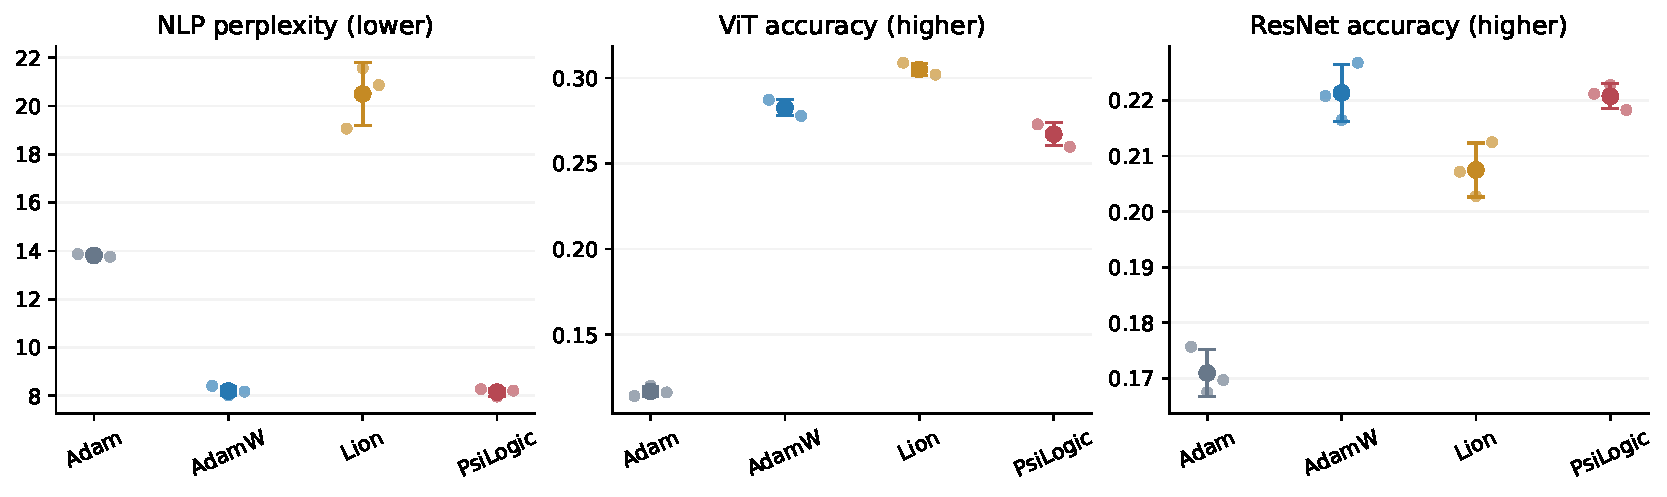
\includegraphics[width=\linewidth]{../../arxiv/figures/later_quality.pdf}
\caption{Later partial snapshot: individual seed points and mean with sample SD for all four optimizers. Accuracy is a fraction. No later diffusion outcomes or learning curves are available.}
\end{figure}

\subsection{Wall time and memory}

\noindent\begin{minipage}{\linewidth}
Table 3. Later run wall time in seconds, mean \(\pm\) sample SD; final column is ratio of means.\par
\begin{center}
\small
\setlength{\tabcolsep}{3pt}
\renewcommand{\arraystretch}{1.15}
\begin{tabularx}{\linewidth}{>{\raggedright\arraybackslash}X>{\raggedright\arraybackslash}X>{\raggedright\arraybackslash}X>{\raggedright\arraybackslash}X>{\raggedright\arraybackslash}X>{\raggedright\arraybackslash}X}
\toprule
\textbf{Arena} & \textbf{Adam} & \textbf{AdamW} & \textbf{Lion} & \textbf{PsiLogic} & \textbf{\path{Psi/AdamW}} \\
\midrule
NLP & 20.49 \(\pm\) 0.17 & 20.22 \(\pm\) 0.07 & 19.90 \(\pm\) 0.07 & 22.22 \(\pm\) 0.18 & 1.099\(\times\) \\
VIT & 113.58 \(\pm\) 1.90 & 114.45 \(\pm\) 3.76 & 112.69 \(\pm\) 1.88 & 117.18 \(\pm\) 0.34 & 1.024\(\times\) \\
RESNET & 36.08 \(\pm\) 0.49 & 35.87 \(\pm\) 0.38 & 35.34 \(\pm\) 0.18 & 37.25 \(\pm\) 0.72 & 1.038\(\times\) \\
\bottomrule
\end{tabularx}
\end{center}

\end{minipage}\par
Overhead relative to AdamW is about 9.9\% for NLP, 2.4\% for ViT, and 3.8\% for ResNet. This supports modest end-to-end overhead in these recorded workloads. It does not show PsiLogic is faster than AdamW, quantify optimizer-only overhead, or isolate fusion's contribution.

\noindent\begin{minipage}{\linewidth}
Table 4. Peak allocated GPU memory in MiB (bytes divided by 1024 squared), mean \(\pm\) sample SD. This is not total board usage or reserved memory.\par
\begin{center}
\small
\setlength{\tabcolsep}{3pt}
\renewcommand{\arraystretch}{1.15}
\begin{tabularx}{\linewidth}{>{\raggedright\arraybackslash}X>{\raggedright\arraybackslash}X>{\raggedright\arraybackslash}X>{\raggedright\arraybackslash}X>{\raggedright\arraybackslash}X}
\toprule
\textbf{Peak allocated MiB} & \textbf{Adam} & \textbf{AdamW} & \textbf{Lion} & \textbf{PsiLogic} \\
\midrule
NLP & 458.4 \(\pm\) 0.1 & 458.4 \(\pm\) 0.1 & 446.0 \(\pm\) 0.1 & 458.6 \(\pm\) 0.1 \\
VIT & 5491.9 \(\pm\) 5.4 & 5492.6 \(\pm\) 3.3 & 5164.4 \(\pm\) 5.3 & 5497.2 \(\pm\) 4.2 \\
RESNET & 857.3 \(\pm\) 0.4 & 855.6 \(\pm\) 0.4 & 812.7 \(\pm\) 0.4 & 857.8 \(\pm\) 0.4 \\
\bottomrule
\end{tabularx}
\end{center}

\end{minipage}\par
Within later arenas, PsiLogic and AdamW have similar allocations. Lion uses less memory. There is no demonstrated memory advantage for PsiLogic; the large cross-snapshot ViT memory change is unexplained by saved metadata.

\begin{figure}[!htbp]
\centering
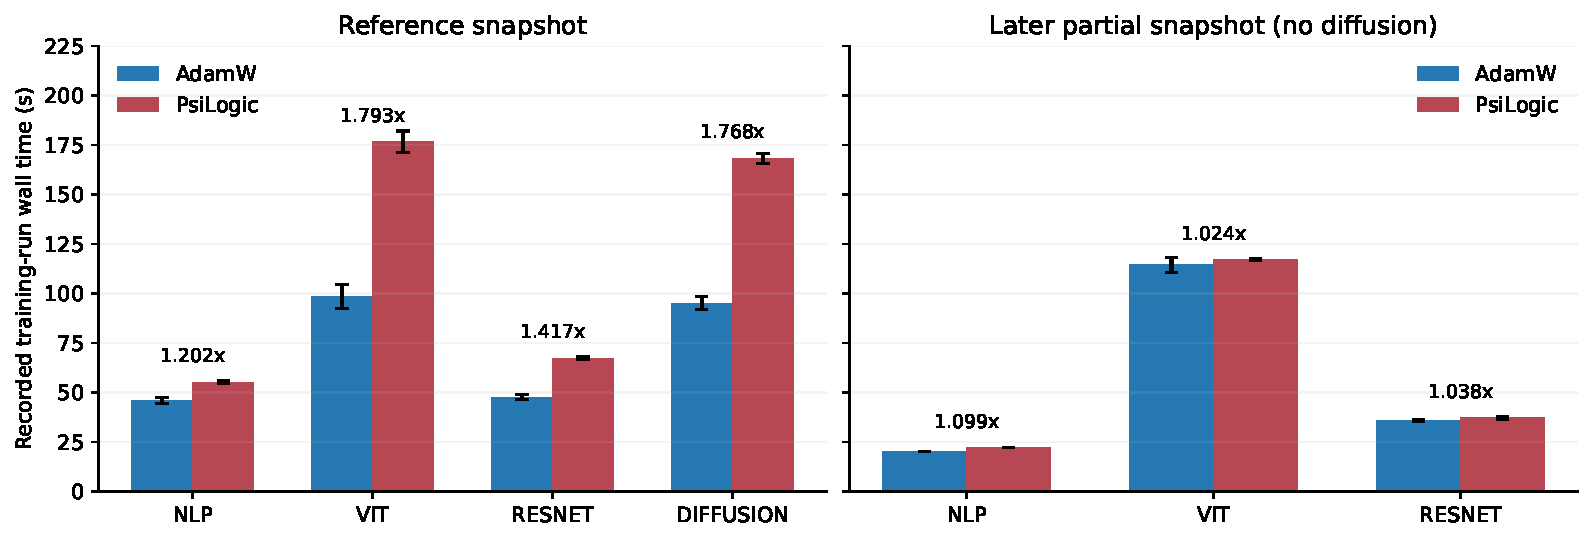
\includegraphics[width=\linewidth]{../../arxiv/figures/wall_time_snapshots.pdf}
\caption{Recorded wall time for AdamW and PsiLogic by snapshot. Bars show means, error bars sample SD, and labels ratios of means. Environments and some selected rates differ; no later diffusion measurement exists.}
\end{figure}

\subsection{Paired comparisons and rates}

The saved optimizer-only profile gives a different cost picture. Its CUDA workload has 202,506 parameters in 50 tensors. The accompanying profiling script compares against foreach AdamW. The saved file reports one median per method, without repeated-run uncertainty or raw timing samples:

\begin{center}
\small
\setlength{\tabcolsep}{3pt}
\renewcommand{\arraystretch}{1.15}
\begin{tabularx}{\linewidth}{>{\raggedright\arraybackslash}X>{\raggedright\arraybackslash}X>{\raggedright\arraybackslash}X}
\toprule
\textbf{Method} & \textbf{Saved median step (ms)} & \textbf{Ratio to AdamW} \\
\midrule
AdamW & 0.603 & 1.00\(\times\) \\
PsiLogic (foreach) & 4.986 & 8.27\(\times\) \\
PsiLogic (fused) & 1.371 & 2.27\(\times\) \\
\bottomrule
\end{tabularx}
\end{center}

Fusion is much faster than PsiLogic's foreach path on this small workload, but the fused step is still about 2.27 times the AdamW step. That is compatible with a small full-training overhead when \path{forward/backward} work dominates, although this separate microbenchmark does not establish the optimizer's share of the three arena runtimes. The saved run note is dated 24 September 2026. Its availability check for Triton supports the intended fused evaluation, but does not replace per-run backend traces or provide a matched comparison with the older environment.

\noindent\begin{minipage}{\linewidth}
Table 5. Later primary-quality tests, raw p / Holm-adjusted p, across nine comparisons. Direction follows Table 1.\par
\begin{center}
\small
\setlength{\tabcolsep}{3pt}
\renewcommand{\arraystretch}{1.15}
\begin{tabularx}{\linewidth}{>{\raggedright\arraybackslash}X>{\raggedright\arraybackslash}X>{\raggedright\arraybackslash}X>{\raggedright\arraybackslash}X}
\toprule
\textbf{Arena} & \textbf{vs Adam raw / Holm} & \textbf{vs AdamW raw / Holm} & \textbf{vs Lion raw / Holm} \\
\midrule
NLP & 0.000275 / 0.00248 & 0.443 / 0.886 & 0.00446 / 0.0235 \\
VIT & 0.000882 / 0.00706 & 0.00735 / 0.0294 & 0.00338 / 0.0235 \\
RESNET & 0.00336 / 0.0235 & 0.902 / 0.902 & 0.0843 / 0.253 \\
\bottomrule
\end{tabularx}
\end{center}

\end{minipage}\par
\noindent\begin{minipage}{\linewidth}
Table 6. Later selected base learning rates.\par
\begin{center}
\small
\setlength{\tabcolsep}{3pt}
\renewcommand{\arraystretch}{1.15}
\begin{tabularx}{\linewidth}{>{\raggedright\arraybackslash}X>{\raggedright\arraybackslash}X>{\raggedright\arraybackslash}X>{\raggedright\arraybackslash}X>{\raggedright\arraybackslash}X}
\toprule
\textbf{Arena} & \textbf{Adam} & \textbf{AdamW} & \textbf{Lion} & \textbf{PsiLogic} \\
\midrule
NLP & 0.000316 & 0.000316 & 0.000316 & 0.000316 \\
VIT & 3.16e-05 & 3.16e-05 & 1e-05 & 3.16e-05 \\
RESNET & 0.0001 & 0.000316 & 0.0001 & 0.000316 \\
\bottomrule
\end{tabularx}
\end{center}

\end{minipage}\par
\section{Historical reference outcomes}

These four-arena results are the reference experiment reported in the original arXiv preprint \citep{psilogic2026preprint}. They are retained here with recalculated statistics, separately from the quality associated with later timing.

\noindent\begin{minipage}{\linewidth}
Table 7. Reference primary metrics, mean \(\pm\) sample SD; bold is best mean.\par
\begin{center}
\small
\setlength{\tabcolsep}{3pt}
\renewcommand{\arraystretch}{1.15}
\begin{tabularx}{\linewidth}{>{\raggedright\arraybackslash}X>{\raggedright\arraybackslash}X>{\raggedright\arraybackslash}X>{\raggedright\arraybackslash}X>{\raggedright\arraybackslash}X}
\toprule
\textbf{Primary metric} & \textbf{Adam} & \textbf{AdamW} & \textbf{Lion} & \textbf{PsiLogic} \\
\midrule
NLP perplexity (lower) & 13.66 \(\pm\) 0.22 & 8.17 \(\pm\) 0.08 & 21.04 \(\pm\) 1.41 & \textbf{7.79 \(\pm\) 0.18} \\
ViT accuracy (higher) & 0.0787 \(\pm\) 0.0035 & 0.2229 \(\pm\) 0.0024 & 0.2127 \(\pm\) 0.0018 & \textbf{0.2444 \(\pm\) 0.0060} \\
ResNet accuracy (higher) & 0.1716 \(\pm\) 0.0044 & 0.2192 \(\pm\) 0.0052 & 0.2045 \(\pm\) 0.0070 & \textbf{0.2221 \(\pm\) 0.0014} \\
Diffusion MSE (lower) & \textbf{0.01987 \(\pm\) 0.00006} & 0.01987 \(\pm\) 0.00006 & 0.02175 \(\pm\) 0.00025 & 0.02009 \(\pm\) 0.00045 \\
\bottomrule
\end{tabularx}
\end{center}

\end{minipage}\par
\noindent\begin{minipage}{\linewidth}
Table 8. Recalculated reference tests, raw p / adjusted p across 12 comparisons.\par
\begin{center}
\small
\setlength{\tabcolsep}{3pt}
\renewcommand{\arraystretch}{1.15}
\begin{tabularx}{\linewidth}{>{\raggedright\arraybackslash}X>{\raggedright\arraybackslash}X>{\raggedright\arraybackslash}X>{\raggedright\arraybackslash}X}
\toprule
\textbf{Arena} & \textbf{vs Adam raw / Holm} & \textbf{vs AdamW raw / Holm} & \textbf{vs Lion raw / Holm} \\
\midrule
NLP & 0.000823 / 0.00906 & 0.0255 / 0.153 & 0.00394 / 0.0394 \\
VIT & 0.000518 / 0.00622 & 0.0465 / 0.232 & 0.0174 / 0.122 \\
RESNET & 0.00439 / 0.0395 & 0.512 / 1 & 0.0586 / 0.235 \\
DIFFUSION & 0.435 / 1 & 0.435 / 1 & 0.00503 / 0.0403 \\
\bottomrule
\end{tabularx}
\end{center}

\end{minipage}\par
These replace the old unadjusted Welch significance claims. Mean ordering is unchanged; inference must follow the recalculated tests rather than old stars. Reference means favor PsiLogic in NLP and ViT, give a small ResNet difference from AdamW, and slightly worse diffusion MSE than \path{Adam/AdamW.} None of the four primary comparisons against AdamW meets the adjusted 0.05 threshold: adjusted p is 0.153 for NLP, 0.232 for ViT, and 1 for ResNet and diffusion. These data therefore do not establish a corrected quality advantage over AdamW, including on diffusion.

\noindent\begin{minipage}{\linewidth}
Table 9. Reference run wall time in seconds and ratio of means.\par
\begin{center}
\small
\setlength{\tabcolsep}{3pt}
\renewcommand{\arraystretch}{1.15}
\begin{tabularx}{\linewidth}{>{\raggedright\arraybackslash}X>{\raggedright\arraybackslash}X>{\raggedright\arraybackslash}X>{\raggedright\arraybackslash}X>{\raggedright\arraybackslash}X>{\raggedright\arraybackslash}X}
\toprule
\textbf{Arena} & \textbf{Adam} & \textbf{AdamW} & \textbf{Lion} & \textbf{PsiLogic} & \textbf{\path{Psi/AdamW}} \\
\midrule
NLP & 46.56 \(\pm\) 1.38 & 45.94 \(\pm\) 1.59 & 38.19 \(\pm\) 7.36 & 55.23 \(\pm\) 0.83 & 1.202\(\times\) \\
VIT & 95.18 \(\pm\) 8.85 & 98.54 \(\pm\) 5.89 & 98.57 \(\pm\) 5.59 & 176.73 \(\pm\) 5.36 & 1.793\(\times\) \\
RESNET & 45.26 \(\pm\) 1.09 & 47.59 \(\pm\) 1.27 & 46.13 \(\pm\) 1.46 & 67.44 \(\pm\) 0.64 & 1.417\(\times\) \\
DIFFUSION & 94.21 \(\pm\) 0.95 & 95.20 \(\pm\) 3.27 & 91.62 \(\pm\) 1.67 & 168.32 \(\pm\) 2.59 & 1.768\(\times\) \\
\bottomrule
\end{tabularx}
\end{center}

\end{minipage}\par
Reference ratios are about 1.20\(\times\), 1.79\(\times\), 1.42\(\times\), and 1.77\(\times\) for NLP, ViT, ResNet, and diffusion. They describe that environment, not later partial measurements. The difference documents an observed cost change without attributing all of it to fusion.

\begin{figure}[!htbp]
\centering
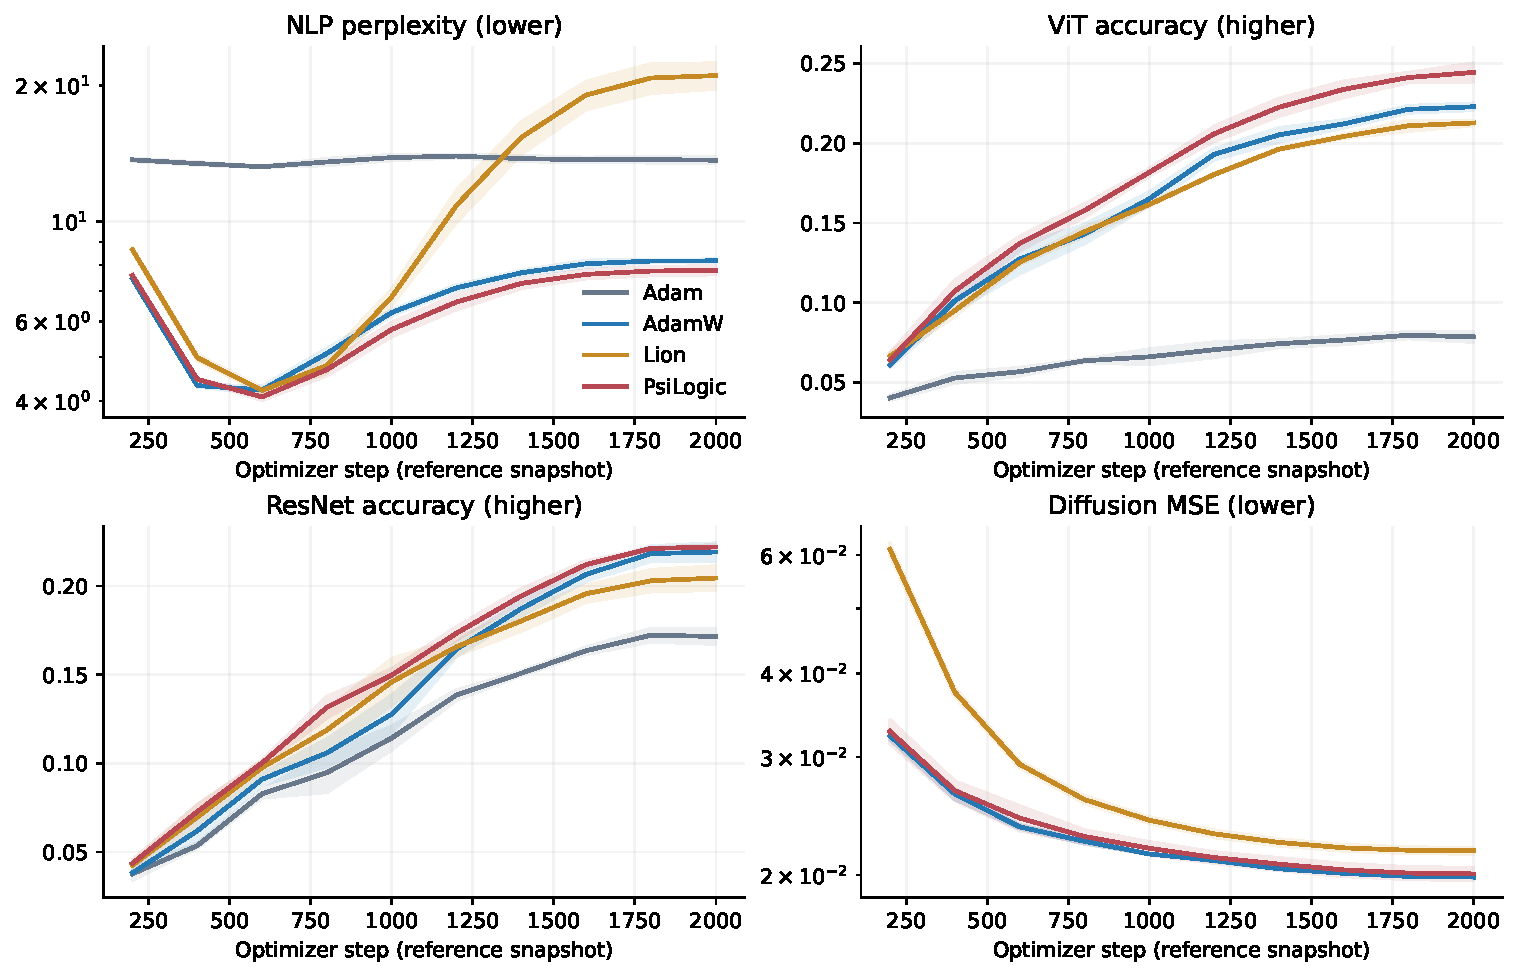
\includegraphics[width=\linewidth]{../../arxiv/figures/reference_learning_curves.pdf}
\caption{Historical reference validation curves regenerated from steps.csv. Lines show means and bands sample SD across three seeds at recorded steps. NLP and diffusion axes are logarithmic. These are not later curves or new training measurements of current source.}
\end{figure}

\section{Discussion and limitations}

The clearest engineering observation is smaller relative full-run overhead in the later snapshot. This coexists with a 2.27-fold optimizer-step cost in the separate saved microbenchmark; the two measurements answer different questions. Quality is less consistent: the older NLP and ViT advantages are not both present later. Software, selected rates, unrecorded \path{architecture/configuration} details, and possible implementation changes remain candidate explanations. Measurements do not isolate these factors or separate cancellation from preprocessing and presets.

Other exploratory NLP follow-ups and older experiments exist. We do not pool them because their settings differ. This is a retrospective report in a project with multiple experiments, not preregistered confirmation. Unit tests establish software properties under tested conditions, not better generalization.

Evidence is limited to three seeds per combination, small models, and short configured budgets. There is no later diffusion outcome, later step history, matched time-to-quality analysis, or external replication established by these artifacts. The convergence theorem in Section~\ref{sec:convergence} applies under its stated restrictions; it does not certify the finite-precision benchmark configurations or explain their quality ordering. Exact training commits, resolved settings, and backend traces are absent. Validation used for LR selection is not an untouched test set. Equal LR candidate counts do not equalize all search effort.

The detector measures relative norm changes and disagreement, not curvature, noise variance, or proof a step is harmful. Its baseline sigmoid value allows damping under steady gradients. Small gradients do not guarantee zero damping. Secondary decay is separate, and epsilon placement makes the zero-cancellation limit different from standard AdamW.

A controlled follow-up should pin code, architecture, data processing, effective batch, precision, and environment; record resolved arguments and backend; compare execution paths under matching settings; and repeat all four tasks with more seeds. Ablations should separately disable cancellation, preprocessing, and secondary decay. Fixed-step quality and time to a prespecified target should both be reported, including unsuccessful runs. These are proposed experiments, not completed evidence.

\section{Reproducing this revision}

The empirical source is \path{PAPER.md}; the theoretical source is \path{research/convergence/manuscript.tex}. The combined article is assembled by \path{research/unified/build.py}. Tables, figures, paired tests, and file hashes are derived from saved measurements:

\begin{Verbatim}[fontsize=\small]
python scripts/paper_results.py
python scripts/build_arxiv_pdf.py
python3 research/unified/build.py
\end{Verbatim}

Analysis requires NumPy, SciPy, and Matplotlib; PDF compilation requires pdflatex or the repository's Tectonic executable. The combined output is \path{output/pdf/paper_unified.pdf}, with editable LaTeX and a shared bibliography in \path{research/unified/}. The standalone empirical build still writes \path{output/pdf/paper.pdf} and its original copies. Analysis and provenance hashes are in \path{arxiv/generated.} Hashes identify analyzed files, not unknown training revisions. Source CSVs remain unchanged. No training or downloads occur during this analysis.

For scholarly citation of PsiLogic, use the original arXiv preprint \citep{psilogic2026preprint}: arXiv:2607.16268, \url{https://arxiv.org/pdf/2607.16268}, article DOI \url{https://doi.org/10.48550/arXiv.2607.16268}. The Zenodo software record \citep{psilogicsoftware} is a supplementary reference for code and artifacts. The revised equations and reanalysis in this local manuscript are dated separately from the original arXiv version.

To evaluate the current update, install benchmark dependencies and prepare datasets as documented in \path{benchmark/README.md.} Record the source revision and resolved arguments before starting:

\begin{Verbatim}[fontsize=\small]
pip install -e ".[benchmark,cuda]"
pip install -r benchmark/requirements.txt
cd benchmark
python -m fairbench --data-root ./data --output-dir results/current_rerun
\end{Verbatim}

This starts a current-default experiment, not a reconstruction of unspecified historical settings. The same optimizer name alone does not make an older table reproducible.

\section{Conclusion}

PsiLogic adds bounded tensor-wise damping around an Adam-style direction, with optional preprocessing, secondary decay, and Lion mode. The equations include details that change its mathematics. Later H100 measurements show 2.4-9.9\% additional recorded run time relative to AdamW across three tasks, near-AdamW NLP and ResNet means, and worse ViT accuracy. The separate optimizer-only microbenchmark still costs 2.27\(\times\) AdamW for fused PsiLogic. Older four-task outcomes remain separate. These findings justify controlled evaluation, not a universal quality claim or a claim that historical tables validate every detail of today's code. The full-detector Adam analysis proves deterministic stationarity and conditional stochastic bounds under explicit restrictions; the counterexamples and the conservative sufficient step bound delimit what those results establish. Ten checked Lean lemmas verify a scalar algebraic core, while the complete convergence theorem remains an informal mathematical proof.


\clearpage
\appendix
\section{Later per-seed primary outcomes}\label{app:empirical-a}

Accuracy is a fraction; tests use seed values before rounding.

\begin{center}
\small
\setlength{\tabcolsep}{3pt}
\renewcommand{\arraystretch}{1.15}
\begin{tabularx}{\linewidth}{>{\raggedright\arraybackslash}X>{\raggedright\arraybackslash}X>{\raggedright\arraybackslash}X>{\raggedright\arraybackslash}X>{\raggedright\arraybackslash}X}
\toprule
\textbf{Arena / seed} & \textbf{Adam} & \textbf{AdamW} & \textbf{Lion} & \textbf{PsiLogic} \\
\midrule
NLP / 0 & 13.86950 & 8.40920 & 19.05928 & 8.27578 \\
NLP / 1 & 13.81303 & 8.02130 & 21.56638 & 7.96639 \\
NLP / 2 & 13.75750 & 8.17168 & 20.86497 & 8.21472 \\
VIT / 0 & 0.11420 & 0.28720 & 0.30890 & 0.27290 \\
VIT / 1 & 0.12020 & 0.28260 & 0.30390 & 0.26880 \\
VIT / 2 & 0.11630 & 0.27780 & 0.30190 & 0.25980 \\
RESNET / 0 & 0.17570 & 0.22080 & 0.20720 & 0.22120 \\
RESNET / 1 & 0.16750 & 0.21650 & 0.20280 & 0.22280 \\
RESNET / 2 & 0.16970 & 0.22680 & 0.21250 & 0.21830 \\
\bottomrule
\end{tabularx}
\end{center}

\section{Reference selected rates}\label{app:empirical-b}

\begin{center}
\small
\setlength{\tabcolsep}{3pt}
\renewcommand{\arraystretch}{1.15}
\begin{tabularx}{\linewidth}{>{\raggedright\arraybackslash}X>{\raggedright\arraybackslash}X>{\raggedright\arraybackslash}X>{\raggedright\arraybackslash}X>{\raggedright\arraybackslash}X}
\toprule
\textbf{Arena} & \textbf{Adam} & \textbf{AdamW} & \textbf{Lion} & \textbf{PsiLogic} \\
\midrule
NLP & 0.000316 & 0.000316 & 0.000316 & 0.000316 \\
VIT & 3.16e-05 & 0.000316 & 0.0001 & 0.000316 \\
RESNET & 0.0001 & 0.000316 & 0.0001 & 0.000316 \\
DIFFUSION & 0.001 & 0.001 & 0.0001 & 0.001 \\
\bottomrule
\end{tabularx}
\end{center}

\section{Reference per-seed primary outcomes}\label{app:empirical-c}

\begin{center}
\small
\setlength{\tabcolsep}{3pt}
\renewcommand{\arraystretch}{1.15}
\begin{tabularx}{\linewidth}{>{\raggedright\arraybackslash}X>{\raggedright\arraybackslash}X>{\raggedright\arraybackslash}X>{\raggedright\arraybackslash}X>{\raggedright\arraybackslash}X}
\toprule
\textbf{Arena / seed} & \textbf{Adam} & \textbf{AdamW} & \textbf{Lion} & \textbf{PsiLogic} \\
\midrule
NLP / 0 & 13.89225 & 8.18040 & 19.46536 & 7.87066 \\
NLP / 1 & 13.64020 & 8.09092 & 21.46757 & 7.58325 \\
NLP / 2 & 13.44957 & 8.24811 & 22.18221 & 7.91506 \\
VIT / 0 & 0.07750 & 0.22550 & 0.21440 & 0.23760 \\
VIT / 1 & 0.08260 & 0.22220 & 0.21080 & 0.24680 \\
VIT / 2 & 0.07590 & 0.22090 & 0.21300 & 0.24880 \\
RESNET / 0 & 0.17510 & 0.21940 & 0.20240 & 0.22090 \\
RESNET / 1 & 0.16660 & 0.21400 & 0.19890 & 0.22360 \\
RESNET / 2 & 0.17300 & 0.22430 & 0.21230 & 0.22170 \\
DIFFUSION / 0 & 0.01985 & 0.01985 & 0.02169 & 0.02004 \\
DIFFUSION / 1 & 0.01982 & 0.01982 & 0.02153 & 0.01967 \\
DIFFUSION / 2 & 0.01993 & 0.01993 & 0.02202 & 0.02057 \\
\bottomrule
\end{tabularx}
\end{center}
\clearpage
\bibliographystyle{unsrtnat}
\bibliography{references}
\end{document}
